\documentclass{article}
\usepackage{graphicx} % Required for inserting images
\usepackage{tikz}
\usetikzlibrary{decorations.pathreplacing}
\usepackage{physics}
\usepackage{amsmath}
\usepackage{adjustbox}
\usepackage{float}
\usepackage{bm}
\usepackage[backend=biber,style=numeric]{biblatex}
\addbibresource{ref.bib}
\usepackage{hyperref}


\title{Pressure and Fluid Flow}
\author{Sandeep Kanekal}
\date{March 2024}

\begin{document}

\maketitle
\section*{Abstract}
This document is the result of an independent study, which was performed in order to understand the fundamental principles of fluid flow. Motivated to quantify fluid flow, I approached it from the first principle that fluids flow from areas of high pressure to low pressure.
From this point, I derived a few relations for pressure gradients, acceleration, continuity of mass, and momentum conservation, and then continued to extend the argument to account for viscous effects for Newtonian fluids. Subsequently, angular momentum and vorticity were added to the document.

Highlights:
\begin{itemize}
    \item \hyperref[eq:continuity]{Continuity Equation (Eq.~\ref*{eq:continuity})}
    \item \hyperref[eq:bernoulli]{Bernoulli’s Equation (Eq.~\ref*{eq:bernoulli})}
    \item \hyperref[eq:inviscid]{Inviscid Flow Equation (Eq.~\ref*{eq:inviscid})}
    \item \hyperref[eq:pflux]{Momentum Flux (Eq.~\ref*{eq:pflux})}
    \item \hyperref[eq:stress_tensor]{Stress Matrix (Eq.~\ref*{eq:stress_tensor})}
    \item \hyperref[eq:navier_stokes]{Force Equation (Eq.~\ref*{eq:navier_stokes})}
    \item \hyperref[eq:viscous_entropy]{Viscous Entropy Equation (Eq.~\ref*{eq:viscous_entropy})}
    \item \hyperref[eq:vorticity]{Vorticity Equation (Eq.~\ref*{eq:vorticity})}
    \item \hyperref[eq:angpflux]{Angular Momentum Flux (Eq.~\ref*{eq:angpflux})}
    \item \hyperref[eq:turbulence]{Turbulence Equation} (Eq.~\ref*{eq:turbulence})
\end{itemize}

\pagebreak
\tableofcontents
\pagebreak

\section{Introduction}
Fluid flow occurs due to a pressure gradient. The flow aims to attain the equilibrium state, that is, to minimise the pressure gradient. That is why a fluid flows from an area of high pressure to that of low pressure. With this simple observation in mind, I wish to find a deeper understanding of fluid mechanics.

I would also like to mention that in order to develop this document, I usually refer to the index of a textbook, so that I can get the initial idea upon which I perform my analysis and study. The mathematics and intuition is done independently unless I state that I have referred to external sources.

\section{The Pressure Gradient}
Consider a cylinder with area $A(y)$, height $h$ filled with some fluid of density $\rho(y)$. We wish to find $\dv{P}{y}$, the pressure gradient.

\begin{figure}[H]
\centering
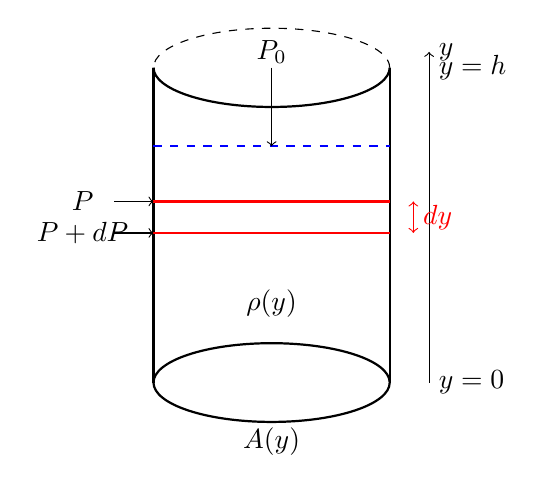
\begin{tikzpicture}
        % Draw the cylinder
        \draw[thick] (0,0) ellipse (1.5 and 0.5);
        \draw[thick] (-1.5,0) -- (-1.5,4);
        \draw[thick] (1.5,0) -- (1.5,4);
        \draw[thick] (-1.5,4) arc[start angle=180,end angle=360,x radius=1.5, y radius=0.5];
        \draw[dashed] (1.5,4) arc[start angle=0,end angle=180,radius=1.5, y radius=0.5];
        
        % Indicate liquid level
        \draw[dashed,blue,thick] (-1.5,3) -- (1.5,3);
        
        % Indicate y-axis and labels
        \draw[->] (2,0) -- (2,4.2) node[right] {$y$};
        \draw (2,0) node[right] {$y=0$};
        \draw (2,4) node[right] {$y=h$};
        
        % Draw differential element (thicker dy)
        \draw[thick,red] (-1.5,1.9) -- (1.5,1.9);
        \draw[thick,red] (-1.5,2.3) -- (1.5,2.3);
        \draw[<->,red] (1.8,1.9) -- (1.8,2.3) node[midway,right] {$dy$};
        
        % Pressure labels
        \draw[->] (0,4) -- (0,3);
        \node at (0,4.2) {$P_0$};
        
        \draw[->] (-2,2.3) -- (-1.5,2.3);
        \node at (-2.4,2.3) {$P$};
        
        \draw[->] (-2,1.9) -- (-1.5,1.9);
        \node at (-2.4,1.9) {$P + dP$};
        
        % Indicate area A
        \node at (0,-0.75) {$A(y)$};
        
        % Indicate fluid density rho
        \node at (0,1) {$\rho(y)$};
    
    \end{tikzpicture}
\caption{Cylinder with Liquid and Pressure Variation}\label{fig:cylinrical-pressure(1)}
\end{figure}

Note that 
\begin{equation*}
    \dd{\vec{F}} = - \dd{P} \cdot A (\hat{n}) \tag{2.1}
\end{equation*}

The negative sign is because this force acts opposite to a pressure gradient. 
\\
Now, the force acting on the small mass element $\dd{m}$ due to gravity is given by
\begin{equation}
    \dd{\vec{F}} = \dd{m} \cdot g (\hat{n})\tag{2.2}
\end{equation}
Here, $\hat{n}$ is a unit vector pointing in the direction of the force. In this case, $\hat{n} = -\hat{y}$.

From (2.1) and (2.2), it follows that
\begin{equation}
    \dd{m} = -\frac{\dd{P}}{g} A \tag{2.3}
\end{equation}

Note that $\dd{m}$ is also given by
\begin{equation}
    \dd{m} = \rho(y) \, \dd{V} \notag
\end{equation}
or
\begin{equation}
    \dd{m} = \rho(y) A(y) \, \dd{y} \tag{2.4}
\end{equation}

Equating (2.3) and (2.4), we get
\begin{equation}
    \frac{\dd{P}}{g} A(y) = -\rho(y) A(y) \, \dd{y} \notag
\end{equation}
\begin{equation}
    \dv{P}{y} = -\rho(y) g \tag{2.5}
\end{equation}

This result implies that the pressure gradient is independent of the cross-sectional area, which is a remarkable result.

Consider $\rho(y) = \rho_0$ where $\rho_0$ is a constant. Therefore, the pressure gradient is constant.
\begin{equation}
    \dv{P}{y} = -\rho_0 g \notag
\end{equation}
\begin{equation}
    \int_{P_o}^{P(h)} \dd{P} = -\int_0^h \rho_0 g \, \dd{y} \notag
\end{equation}
which is the familiar result
\begin{equation}
    P(h) = P_o - \rho_0 g h \tag{2.6}
\end{equation}
This result is consistent with observation. The pressure is supposed to decrease with height.

I have assumed that the height of the cylinder is negligible compared to the radius of the Earth. If one were to perhaps design a ``space pipe'', one would have to account for the variation of $g$ with height.

\section{Fluid Flow due to Pressure Gradients}
Consider a U-shaped tube with a pressure gradient. Let the flow be from the left to the right and the velocity of the fluid be denoted by $v(y)$. Let $\dv{V}{t}$ denote the flow rate, where $\dd{V}$ is an infinitesimal change in the volume of the fluid. We wish to find an expression for $\dv{V}{t}$ in terms of the pressure gradient.

\begin{figure}[H]
\centering
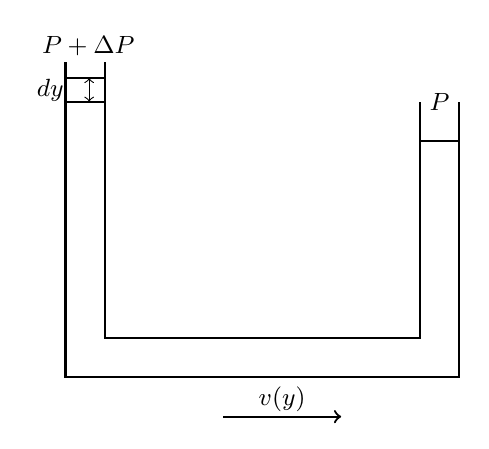
\begin{tikzpicture}
        % Outer boundary of the U-tube (shifted by -0.5)
        \draw[thick] (-2,1.5) -- (-2,-2.5) -- (3,-2.5) -- (3,1);
        
        % Inner boundary of the U-tube (shifted by -0.5)
        \draw[thick] (-1.5,1.5) -- (-1.5,-2) -- (2.5,-2) -- (2.5,1);
        
        % Liquid levels (shifted by -0.5)
        \draw[thick] (-2,1) -- (-1.5,1);
        \draw[thick] (-2,1.3) -- (-1.5,1.3);
        \draw[thick] (3,0.5) -- (2.5,0.5);
        
        % Pressure labels (shifted by -0.5)
        \node[left] at (-1,1.7) {\small $P + \Delta P$};
        \node[right] at (2.5,1) {\small $P$};
        
        % Indicate small height dy (shifted by -0.5)
        \draw[<->] (-1.7,1) -- (-1.7,1.3);
        \node[left] at (-1.9,1.15) {\small $dy$};
        
        % Flow direction (shifted by -0.5)
        \draw[->, thick] (0,-3) -- (1.5,-3);
        \node[below] at (0.75,-2.5) {\small $v(y)$};
        
    \end{tikzpicture}
\caption{U-shaped Tube with Pressure Difference}\label{fig:U-tube(2)}
\end{figure}

Substituting $\mathrm{d}m = \rho \mathrm{d}V$ in equation (2.3), we arrive at the following expression for $\mathrm{d}V$
\begin{equation}
    \dd{V} = -\frac{A(y)}{\rho(y) g} \, \dd{P} \tag{3.1}
\end{equation}
The negative sign is because the volume (on the left side of the tube) is decreasing. Following this, we get
\begin{equation}
    \dv{V}{t} = -\frac{A(y)}{\rho(y) g} \dv{P}{t} \tag{3.2}
\end{equation}
By the chain rule, we arrive at the following equation.
\begin{equation}
    \dv{V}{t} = -\frac{A(y)}{\rho(y) g} \dv{P}{y} \dv{y}{t} \tag{3.3}
\end{equation}
Note that $\dv{y}{t} = v(y)$. Therefore, the equation simplifies to the following.
\begin{equation}
    \dv{V}{t} = -\frac{A(y) v(y)}{\rho(y) g} \dv{P}{y} \tag{3.4}
\end{equation}
Substituting result (2.5) in (3.4), we get the following equation.
\begin{equation}
    \dv{V}{t} = -A(y) v(y) \tag{3.5}
\end{equation}
This result is precisely the equation of continuity. This result is also consistent with observation. If \(v(y)\) is positive, i.e., flowing out of the container, the volume would decrease with time.
\\
Intuitively, it must be true that $\dv{V}{t}$ is a constant throughout the tube. If not, there would be more fluid coming out of the other end than supplied or vice versa.

Therefore,
\begin{equation}
    A_1 v_1 = A_2 v_2 \tag{3.6}
\end{equation}
holds throughout the tube.

\section{Assumptions made}
This argument that I have made is not without limitations. Here are the assumptions.
\begin{enumerate}
    \item The fluid is assumed to be ideal.
    \item The fluid is assumed to have no viscous drag.
    \item Laminar flow of the fluid is assumed. That is, there is no turbulent flow at all.
\end{enumerate}

I wish to improve my arguments by accounting for the above-stated assumptions, which generally are non-negligible.

\section{Extending to general cases}
In the previous arguments that were made. I had assumed that the pressure was due to gravity. In order to make a model that is more general, I will now assume a fluid in a negligible gravitational field that has a pressure gradient acting along it. I would also like to extend the argument to all 3 spatial dimensions.

\subsection{Acceleration}
From (2.5), we can change $g$ with $\vec{a}$ to get the acceleration caused by a pressure gradient. That is:
\begin{align*}
    a_x &= -\frac{1}{\rho} \pdv{P}{x} \\
    a_y &= -\frac{1}{\rho} \pdv{P}{y} \\
    a_z &= -\frac{1}{\rho} \pdv{P}{z}
\end{align*}
The negative signs indicate that acceleration is positive down a pressure gradient.

\begin{align*}
    \vec{a} &= a_x \hat{x} + a_y \hat{y} + a_z \hat{z} \\
           &= -\frac{1}{\rho} \qty( \pdv{P}{x} \hat{x} + \pdv{P}{y} \hat{y} + \pdv{P}{z} \hat{z} ) \\
           &= -\frac{1}{\rho} \nabla P \tag{5.1.1}
\end{align*}

\subsection{Force}
By applying Newton's law of motion, we can find the force acting on the fluid due to the pressure gradient.
\begin{align*}
    \vec{F} &= m \vec{a} \\
           &= -\frac{m}{\rho} \nabla P \hspace{2cm} \text{From equation (5.1.1)}\\
           &= -V \nabla P
\end{align*}

This result implies that the force acting on a fluid depends on the volume of the fluid as well. This result, however, may not be very useful because of its dependence on volume. Therefore, I define another quantity $\vec{f} = \vec{F} / V$ (Force per unit volume).

\begin{equation}
    \vec{f} = -\nabla P
    \tag{5.2.1}
\end{equation}

\subsection{Work and Energy}
Work is defined as the line integral of the force field along a path.
\begin{align*}
    W &= \int_\Gamma \vec{F} \cdot \dd{\vec{r}} \\
    w &= \frac{W}{V} = \int_\Gamma \vec{f} \cdot \dd{\vec{r}} \\
      &= -\int_A^B \nabla P \cdot \dd{\vec{r}} = -\int_A^B \dd{P} \quad \text{(By Gradient Theorem)} \\
      &= P(A) - P(B) = -\Delta P \tag{5.3.1}
\end{align*}

Note that the work done is positive when the fluid is moving down the pressure gradient.

Similarly, work per unit mass can also be defined. The result is
\[
    \frac{W}{m} = -\frac{1}{\rho} \Delta P
\]


\section{Continuity}

\subsection{Conservation of Mass}
The result, which I had derived earlier, i.e., $\dv{V}{t} = $ constant does not capture the entire picture. Considering the same conditions as in Fig 3, it would be better to consider mass rate instead.

\begin{align*}
    \dot{m} &= \dv{(\rho V)}{t} \\
            &= \rho \dot{V} = \rho A v
\end{align*}

This relates the mass rate to the cross-sectional area of the pipe. For any fluid with constant $\rho$, one can conclude that the volume flow rate will be constant. However, if the density is not constant, the volume flow rate will not be constant throughout the tube.

\textbf{Corollary:} $\dot{V}$ is constant if the fluid is of uniform density.

\subsection{Equation of Continuity}
Consider a system containing a fluid with some fluid flowing into or out of it. What would the equation of continuity look like?

First, we consider the case where there is no net flow inward or outward — an isolated system.

\begin{gather*}
    m = \int_V \rho\, \mathrm{d}V \\
    \intertext{Differentiating with respect to time:} \\
    \dv{m}{t} = \dv{t} \int_V \rho\, \mathrm{d}V \\
    \intertext{As the volume element does not change with time, the derivative can be taken inside the integral}\\
    \dv{m}{t} = \int_V \pdv{\rho}{t}\, \mathrm{d}V \\
    \text{Since the system is isolated, the mass change rate is zero:} \\
    \int_V \pdv{\rho}{t}\, \mathrm{d}V = 0
\end{gather*}

Now, if there is a net flow of fluid inwards or outwards (at any point), the mass must still be conserved. Therefore, some other factor must affect the density of the fluid if flow occurs.

Let $\vec{v}$ denote the velocity vector field. We now consider the volume flux, defined as the volume of fluid flowing through a surface of unit area per unit time. For an area element $\mathrm{d}\vec{S}$, the flux is given by
\[
    \phi_V = \int_S \vec{v} \cdot \mathrm{d}\vec{S}
\]
Therefore, the mass flux is
\[
    \phi_m = \int_S \rho \vec{v} \cdot \mathrm{d}\vec{S}
\]

By Gauss' Divergence Theorem, we can express this as a volume integral:
\[
    \phi_m = \int_V \nabla \cdot{(\rho \vec{v})}\, \mathrm{d}V
\]

Applying conservation of mass:
\begin{align*}
    \dv{m}{t} &= -\phi_m = -\int_V \nabla \cdot{(\rho \vec{v})}\, \mathrm{d}V \\
    \dv{}{t} \int_V \rho\, \mathrm{d}V &= -\int_V \nabla \cdot{(\rho \vec{v})}\, \mathrm{d}V \\
    \int_V \pdv{\rho}{t}\, \mathrm{d}V &= -\int_V \nabla \cdot{(\rho \vec{v})}\, \mathrm{d}V
\end{align*}

Thus,
\[
    \int_V \qty( \pdv{\rho}{t} + \nabla \cdot{(\rho \vec{v})} )\, \mathrm{d}V = 0
\]

Since the mass is conserved and all possible inflow/outflow has been accounted for by the flux term, the integrand must vanish identically for the result to hold generally:
\begin{equation}
    \pdv{\rho}{t} + \nabla \cdot{(\rho \vec{v})} = 0 \tag{6.2.1} \label{eq:continuity}
\end{equation}

The integral version of this equation is given by
\[
    \dv{m}{t} = - \oint \rho \vec{v} \cdot \dd{\vec{A}} \tag{6.2.2}
\]

\(\vec{A}\) refers to the normal area vector.

\subsection{Special Case---incompressible fluid}
Expanding (6.2.1), we get:
\begin{equation*}
    \pdv{\rho}{t} + \rho\, (\nabla \cdot{\vec{v}}) + \vec{v} \cdot \nabla \rho = 0 \tag{6.3.1}
\end{equation*}

An incompressible fluid assumes that the density is uniform and steady. Therefore
\[
    \pdv{\rho}{t} = 0
\]
and
\[
    \pdv{\rho}{i} = 0 \quad (i \in \{x, y, z\}) \implies \nabla \rho = \vec{0}
\]

Therefore, by these assumptions,
\begin{gather*}
    \rho (\nabla \cdot \vec{v}) = 0 \\
    \implies \nabla \cdot \vec{v} = 0
\end{gather*}




\subsection{Discussions}
I had learned about the equation of continuity in electromagnetism lectures and noticed that charges behaved like fluids. Therefore, the form of the equations must be somewhat similar. Essentially, some quantity is conserved when flux is accounted for. In this case, it is mass; in electromagnetism, it is charge. Possibly, heat flow follows a similar equation, as it is dependent on the thermal gradient — in which case, energy is probably conserved (assuming no heat loss occurs).


\section{Energy conservation along a streamline}
In order to find an equation that describes how energy is conserved along a streamline, we will start with simple cases and build up to a general equation.

\subsection{Situation}
Consider a section of a tube with ends A and B having pressures \( P(A) \) and \( P(B) \), and velocities \( v(A) \) and \( v(B) \), respectively. Here, A and B need not correspond to the ends of the tube.

\begin{figure}[H]
\centering
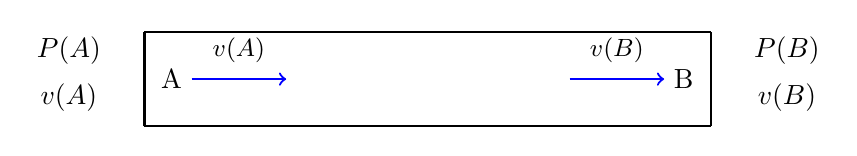
\begin{tikzpicture}[scale=1.2]

    % Tube
    \draw[thick] (0,1) -- (6,1);
    \draw[thick] (0,0) -- (6,0);

    % End A
    \draw[thick] (0,0) -- (0,1);

    % End B
    \draw[thick] (6,0) -- (6,1);

    % Labels
    \node at (0.5,0.5) [left] {A};
    \node at (5.5,0.5) [right] {B};

    \node at (-0.8,0.8) {$P(A)$};
    \node at (-0.8, 0.3) {$v(A)$};
    \node at (6.8,0.8) {$P(B)$};
    \node at (6.8, 0.3) {$v(B)$};

    % Velocity arrows
    \draw[->, thick, blue] (0.5,0.5) -- (1.5,0.5);
    \draw[->, thick, blue] (4.5,0.5) -- (5.5,0.5);

    \node at (1,0.8) {\small $v(A)$};
    \node at (5,0.8) {\small $v(B)$};

    \end{tikzpicture}
\caption{Section of a tube}\label{fig:tube-section(3)}
\end{figure}

Assuming there exists no other force other than the pressure gradient force, we can equate energy at A to be equal to energy at B:\

\[
\frac{1}{2}mv_A^2 + U(A) = \frac{1}{2}mv_B^2 + U(B)
\]

However, the term \( m \) does not make sense for a continuous fluid. Therefore, dividing by the volume at any point, we get:

\begin{equation}
\frac{1}{2}\rho_A v_A^2 + T(A) = \frac{1}{2}\rho_B v_B^2 + T(B) \tag{7.1.1}
\end{equation}

where \( T(r) \) stands for the energy density at point \( r \).

\subsection{Form of the energy density function}
Before finding the form of \( T \), it is required to know the form of \( U \). It helps to know whether \( U \) is the potential energy function of a conservative force or not. As we have found from equation (5.3.1), the work done per unit volume depends only on the endpoints. Therefore, the pressure gradient force is conservative in nature.

Hence, the force can be written as the negative of the gradient of the potential energy function:

\[
\vec{F} = -\nabla U
\]

which implies that
\[
U = -\int_\Gamma \vec{F} \cdot \mathrm{d}\vec{r} = -W
\]

I would like to define the potential energy function at every point. Therefore, a reference point is required. This reference point must satisfy \( U = 0 \), which is possible when \( P = 0 \). Thus, \( U \) is defined as the work done to bring a fluid from zero pressure to a positive pressure.

Therefore,

\[
U(\vec{r}) = -\int_{\vec{r}_\text{ref}}^{\vec{r}} \vec{F} \cdot \mathrm{d}\vec{r}
\]

which implies

\[
T(\vec{r}) = -\int_{\vec{r}_\text{ref}}^{\vec{r}} \vec{f} \cdot \mathrm{d}\vec{r}
\]

From (5.2.1), we have \( \vec{f} = -\nabla P \). Therefore,

\begin{align}
T(\vec{r}) &= \int_{\vec{r}_\text{ref}}^{\vec{r}} \nabla P \cdot \mathrm{d}\vec{r}  = \int_{\vec{r}_\text{ref}}^{\vec{r}} \dd{P} \notag \\
         &= \Delta P \notag \\
         &= P(\vec{r}) - P(\vec{r}_\text{ref}) \notag \\
         &= P(\vec{r}) \tag{7.2.1}
\end{align}

\subsection{The final equation}
Substituting (7.2.1) into (7.1.1), we find the final equation for conservation of energy along a streamline:

\[
\frac{1}{2}\rho_A v_A^2 + P(A) = \frac{1}{2}\rho_B v_B^2 + P(B)
\]

So, the general result can be written as:

\begin{equation}
\frac{1}{2}\rho v^2 + P = \text{constant} \tag{7.3.1} \label{eq:bernoulli}
\end{equation}

If one were to account for gravity, we get the relation:

\begin{equation}
    \frac{1}{2}\rho v^2 + P + \rho g h = \text{constant} \tag{7.3.2}
\end{equation}

where \( h \) is the height from the Earth’s surface. This is precisely Bernoulli's equation. It is important to note that this equation corresponds to every point in the fluid, therefore, it is a local version of the energy conservation equation.

\subsection{Applications}
Some applications include flow out of a hole, change in velocity and pressure when the radius of the pipe changes, and pipes with varying cross-sections. These applications require both the equation of continuity and Bernoulli's equation.

\subsubsection{Flow out of a hole}
\begin{figure}[H]
\centering
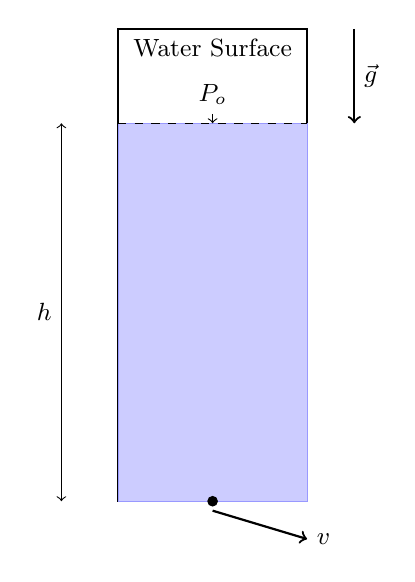
\begin{tikzpicture}[scale=1.2]
    
      % Tank
      \draw[thick] (0,0) rectangle (2,5); % tank walls
      \draw[blue!40, fill=blue!20] (0,0) rectangle (2,4); % water
    
      % Water surface and height label
      \draw[dashed] (0,4) -- (2,4);
      \draw[<->] (-0.6,0) -- (-0.6,4);
      \node[left] at (-0.6,2) {\small $h$};
    
      % Pressure at top
      \node[above] at (1,4.1) {\small $P_o$};
      \draw[->] (1,4.1) -- (1,4); % atmospheric pressure
    
      % Hole and velocity vector
      \filldraw[black] (1,0) circle (0.05); % hole
      \draw[->, thick] (1,-0.1) -- (2,-0.4);
      \node[right] at (2,-0.4) {\small $v$};
    
      % Gravity vector
      \draw[->, thick] (2.5,5) -- (2.5,4);
      \node[right] at (2.5,4.5) {\small $\vec{g}$};
    
      % Water surface label
      \node at (1,4.8) {\small Water Surface};
    
    \end{tikzpicture}
\caption{Flow out of a hole}\label{fig:flow-hole(4)}
\end{figure}

I wish to find an expression for \(v\). Applying Bernoulli's law at the water surface and at the hole, we get the following expression:
\[
    \frac{1}{2} \rho v_\text{surface}^2 + P_\text{surface} + \rho g h = \frac{1}{2} \rho v_\text{hole}^2 + P_\text{hole} + \rho g (0)
\]
As the hole is exposed to the atmosphere, the pressure is equal to the atmospheric pressure. And when the surface is very far from the hole \(v \approx 0\) (If the surface were at infinity, \(v=0\)). Therefore:
\begin{gather}
    \frac{1}{2} \rho v^2 + P_0 = P_0 + \rho g h \notag \\
    \implies v = \sqrt{2gh} \notag
\end{gather}

\subsubsection{Flow in pipes with varying cross-sections}
\begin{figure}[H]
\centering
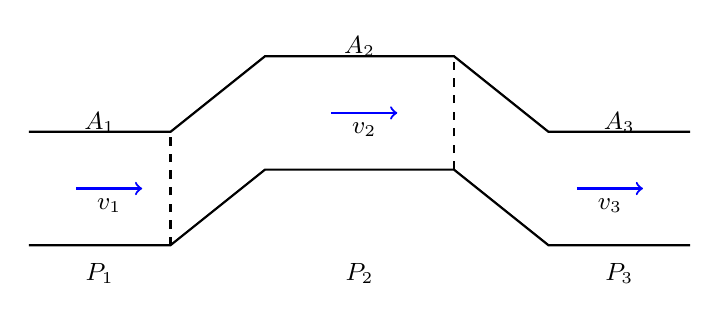
\begin{tikzpicture}[scale=1.2, thick]

  % Pipe walls
  \draw (0,1.2) -- (1.5,1.2) -- (2.5,2) -- (4.5,2) -- (5.5,1.2) -- (7,1.2);
  \draw (0,0) -- (1.5,0) -- (2.5,0.8) -- (4.5,0.8) -- (5.5,0) -- (7,0);

  % Vertical dashed lines (sections)
  \draw[dashed] (1.5,0) -- (1.5,1.2);
  \draw[dashed] (4.5,0.8) -- (4.5,2);

  % Velocity arrows
  \draw[->, blue, thick] (0.5,0.6) -- (1.2,0.6);
  \node[below] at (0.85,0.6) {\small $v_1$};

  \draw[->, blue, thick] (3.2,1.4) -- (3.9,1.4);
  \node[below] at (3.55,1.4) {\small $v_2$};

  \draw[->, blue, thick] (5.8,0.6) -- (6.5,0.6);
  \node[below] at (6.15,0.6) {\small $v_3$};

  % Area labels
  \node at (0.75,1.3) {\small $A_1$};
  \node at (3.5,2.1) {\small $A_2$};
  \node at (6.25,1.3) {\small $A_3$};

  % Pressure labels
  \node at (0.75,-0.3) {\small $P_1$};
  \node at (3.5,-0.3) {\small $P_2$};
  \node at (6.25,-0.3) {\small $P_3$};

\end{tikzpicture}
\caption{Pipe with varying cross sections}\label{fig:cross-section-pipe(5)}
\end{figure}
Firstly, mass is conserved. Therefore:
\[
    \dot{m} = \rho Av = \text{constant}
\]
If the density is uniform, we arrive at the following result:
\[
    Av = \text{constant}
\]

This result can even be derived from the equation of continuity. Assuming incompressibility, that is, $\pdv{\rho}{t} = 0$, we arrive at the following result:
\begin{gather}
    \nabla \cdot{\rho \vec{v}} = 0 \notag \\
    \implies \rho (\nabla \cdot{\vec{v}}) = 0 \quad (\nabla \rho=0) \notag \\
    \implies \nabla \cdot{\vec{v}} = 0 \notag
\end{gather}
By the divergence theorem, we have:
\begin{gather}
    \int_A \vec{v} \cdot \dd{\vec{A}} = 0 \notag \\
    \implies \int_A v \hat{v} \cdot \hat{n} \dd{A} = 0 \notag \\
    \implies Av = \text{constant} \notag
\end{gather}

Applying Bernoulli's equation in areas 1 and 3, we get the following:
\begin{gather}
    \frac{1}{2} \rho v_1^2 + P_1 + \rho g h = \frac{1}{2} \rho v_3^2 + P_3 + \rho g h \notag \\
    \implies \frac{1}{2} \rho v_1^2 + P_1 = \frac{1}{2} \rho v_3^2 + P_3 \notag
\end{gather}

Compactly written, in case of horizontal flow, the following result holds true:
\[
    \frac{1}{2} \rho v^2 + P = \text{constant}
\]
This expression explains why the pressure increases when the velocity decreases in horizontal flow. The opposite holds true as well.


\section{Acceleration as a spatial and temporal derivative}
It is apparent from equation~(3.6) that the velocity can change with the cross-sectional area. That is, the velocity has a spatial variation. Along any streamline, if the area perpendicular to that streamline changes, so does the velocity, that is, there is acceleration. Therefore, the acceleration is not just a derivative with respect to time~\cite{landau}.
\\
Let $\vec{v}$ be a function of the form:

\[
    \vec{v} = \vec{v}(x(t), y(t), z(t), t)
\]

Then, using the chain rule:

\begin{align}
    \dv{\vec{v}}{t} &= \pdv{\vec{v}}{t} + \pdv{\vec{v}}{x} \dv{x}{t} + \pdv{\vec{v}}{y} \dv{y}{t} + \pdv{\vec{v}}{z} \dv{z}{t} \notag \\
    &= \pdv{\vec{v}}{t} + v_x \pdv{\vec{v}}{x} + v_y \pdv{\vec{v}}{y} + v_z \pdv{\vec{v}}{z} \tag{i}
\end{align}

Now, consider the term:

\begin{align}
    (\vec{v} \cdot \nabla) \vec{v} &= \qty((v_x \hat{x} + v_y \hat{y} + v_z \hat{z}) \cdot \qty(\pdv{x} \hat{x} + \pdv{y} \hat{y} + \pdv{z} \hat{z})) \vec{v} \notag \\
    &= \qty(v_x \pdv{x} + v_y \pdv{y} + v_z \pdv{z}) \vec{v} \notag \\
    &= v_x \pdv{\vec{v}}{x} + v_y \pdv{\vec{v}}{y} + v_z \pdv{\vec{v}}{z} \tag{ii}
\end{align}

Substituting (ii) into (i), we obtain:

\begin{equation}
    \vec{a} = \pdv{\vec{v}}{t} + (\vec{v} \cdot \nabla) \vec{v} \tag{8.1}
\end{equation}

From equation (5.2.1), the pressure force is given by $\vec{f} = -\nabla P$. According to Newton’s second law, we also have $\vec{f} = \rho \vec{a}$. Therefore:

\begin{equation}
    \rho \qty[\pdv{\vec{v}}{t} + (\vec{v} \cdot \nabla) \vec{v}] = -\nabla P \tag{8.2}
\end{equation}

\textit{Note:} At this stage, I am not certain whether $\rho \vec{v}$ can always be treated in the same way as $\vec{v}$. I will revise this if necessary.

Now, if the fluid has uniform density, i.e., $\rho = \rho_0$, then:

\begin{equation}
    \rho_0 \qty[\pdv{\vec{v}}{t} + (\vec{v} \cdot \nabla) \vec{v}] = -\nabla P \tag{8.3}
\end{equation}

Dividing both sides by $\rho_0$, we arrive at:

\[
    \vec{a} = -\frac{1}{\rho_0} \nabla P
\]

This is consistent with the earlier derived expression for acceleration. Hence, the previous result is valid only for fluids with constant density, in line with our assumptions.

\section{Momentum}
\subsection{Momentum density}
Momentum density is defined as the derivative of momentum with respect to volume.
\[
    \vec{M} = \dv{\vec{p}}{V} = \dv{(m \vec{v})}{V} = \rho \vec{v} \tag{9.1.1}
\]


\subsection{Force equation}

By Newton's second law:
\[
    \vec{f} = \rho \vec{a} = \rho \dv{\vec{v}}{t}
\]

Now, consider the following
\begin{align}
    \dv{\vec{M}}{t} &= \dv{(\rho \vec{v})}{t} \notag \\
    &= \rho \dv{\vec{v}}{t} + \vec{v} \dv{\rho}{t} \quad \text{(Product rule)} \notag \\
    &= \rho \vec{a} + \vec{v} \dv{\rho}{t} \notag \\
    &= \vec{f} + \vec{v} \dv{\rho}{t} \tag{i}
\end{align}

Now, consider the continuity equation
\begin{gather}
    \pdv{\rho}{t} + \nabla \cdot{(\rho \vec{v})} = 0 \notag \\
    \implies \pdv{\rho}{t} + \rho(\nabla \cdot{\vec{v}}) + \vec{v} \cdot (\nabla \rho) = 0 \notag \\
    \implies \pdv{\rho}{t} + \vec{v} \cdot (\nabla \rho) = -\rho(\nabla \cdot{\vec{v}}) \tag{ii}
\end{gather}

Note that
\begin{align}
    \vec{v} \cdot \nabla \rho &= (v_x \hat{x} + v_y \hat{y} + v_z \hat{z}) \cdot \qty(\pdv{\rho}{x} \hat{x} + \pdv{\rho}{y} \hat{y} + \pdv{\rho}{z} \hat{z}) \notag \\
    &= v_x \pdv{\rho}{x} + v_y \pdv{\rho}{y} + v_z \pdv{\rho}{z} \notag \\
    &= \qty[v_x \pdv{x} + v_y \pdv{y} + v_z \pdv{z}] \rho \equiv (\vec{v} \cdot \nabla) \rho \tag{iii}
\end{align}

Therefore, substituting (iii) in (ii), we get
\begin{gather}
    \pdv{\rho}{t} + (\vec{v} \cdot \nabla) \rho = -\rho(\nabla \cdot{\vec{v}}) \notag \\
    \implies \dv{\rho}{t} = -\rho(\nabla \cdot{\vec{v}}) \tag{iv}
\end{gather}

Substituting (iv) in (i) and rearranging, we get
\begin{gather}
    \vec{f} = \dv{\vec{M}}{t} + \rho \vec{v} (\nabla \cdot{\vec{v}}) \notag \\
    \implies -\nabla P = \dv{\vec{M}}{t} + \rho \vec{v} (\nabla \cdot{\vec{v}}) \notag \\
    \implies \nabla P + \dv{\vec{M}}{t} + \rho \vec{v} (\nabla \cdot{\vec{v}}) = 0 \tag{9.2.1}
\end{gather}
This equation relates the pressure gradient to the derivative of momentum density and the velocity divergence term. It emphasizes how momentum changes due to both local acceleration and volumetric expansion or compression of the fluid. Under the incompressibility assumption, the divergence of velocity is zero:
\[
    \nabla \cdot{\vec{v}} = 0 \quad \text{and} \quad \dv{\rho}{t} = 0
\]

Thus, we get the following result:
\begin{gather}
    \dv{\vec{M}}{t} = -\nabla P \notag \\
    \implies \rho \dv{\vec{v}}{t} + \vec{v} \dv{\rho}{t} = -\nabla P \quad \text{(Product rule)} \notag
\end{gather}
\begin{equation}
        \implies \rho \dv{\vec{v}}{t} = -\nabla P \quad \qty(\dv{\rho}{t} = 0) \tag{9.2.2} \label{eq:inviscid}
\end{equation}

\subsection{Conservation of momentum}
This subsection was added after the section ``Viscosity'' was done and ``Angular momentum'' was being typed, therefore, I would suggest at least completing the viscosity section before reading this. 

The linear momentum is conserved similar to the continuity equation. The rate of change in the momentum along with the flux is equal to the body force acting on the system. Therefore, the equation takes the form
\[
    \pdv{\vec{p}}{t}  + \nabla \cdot (\text{momentum flux term}) = \vec{F}
\]
The momentum flux\cite{landau} term must be of the same dimension as that of force. Therefore
\[
    \dd{\vec{\phi}} = \bm{M} \cdot \dd{\vec{A}}
\]
The terms in the momentum flux include the pressure gradient and the viscous terms. Therefore
\[
    \bm{M} = P\bm{I} - \bm{S}
\]
where $\bm{I}$ is the identity matrix and $\bm{S}$ is the viscous stress matrix. The reason $P\bm{I}$ is taken to be the pressure gradient flux term is because the divergence of this term should be equal to the force density term caused by the pressure gradient. Note that
\begin{align*}
    -\nabla \cdot P\bm{I} &= \begin{pmatrix}
        \partial_x \\ \partial_y \\ \partial_z
    \end{pmatrix} \cdot \begin{pmatrix}
        -P & 0 & 0 \\
        0 & -P & 0 \\
        0 & 0 & -P
    \end{pmatrix} \\
    &= -\begin{pmatrix}
        \displaystyle \pdv{P}{x} \\[1.5em]
        \displaystyle \pdv{P}{y} \\[1.5em ]
        \displaystyle \pdv{P}{z}
    \end{pmatrix} \\
    &= -\nabla P
\end{align*}

By the divergence theorem, the flux can also be expressed as a volume integral, which is
\[
    \vec{\phi} = \iint \bm{M} \cdot \dd{\vec{A}} = \iiint (\nabla \cdot \bm{M}) \dd{V}
\]

Using the following equations
\begin{gather*}
    \pdv{\vec{p}}{t} = \pdv{}{t} \iiint \rho \vec{v} \dd{V} = \iiint \pdv{(\rho \vec{v})}{t} \dd{V}
    \intertext{and}
    \vec{F} = \iiint \vec{f} \dd{V}
\end{gather*}
Leads to
\begin{gather*}
    \iiint \qty[\pdv{(\rho \vec{v})}{t} + \nabla \cdot \bm{M}] \dd{V} = \iiint \vec{f} \dd{V} \\
    \iiint \qty[\pdv{(\rho \vec{v})}{t} + \nabla \cdot \bm{M} - \vec{f}] \dd{V} = 0
    \intertext{For this integral to be equal to zero generally, the integrand must be identically 0}
    \implies \pdv{(\rho \vec{v})}{t} + \nabla \cdot \bm{M} - \vec{f} = 0 \\
    \implies \pdv{(\rho \vec{v})}{t} + \nabla \cdot \bm{M} = \vec{f}
\end{gather*}

If this equation were complete, then the force equation should appear after a few mathematical manipulations. The equation thus expanded becomes:
\begin{gather*}
    \pdv{(\rho \vec{v})}{t}  = -\nabla \cdot {P\bm{I}} + \mu{[\nabla\vec{v} + {(\nabla \vec{v})}^T]} + \vec{f} \\
    \intertext{Assuming incompressibility}
    \rho \pdv{\vec{v}}{t} = -\nabla P + \mu \nabla^2 \vec{v} + \vec{f}
\end{gather*}

However, this is not correct, therefore, there must be a missing term in the momentum flux matrix. This term should be such that the divergence of it should be equal to the convective term in the field derivative of velocity (assuming incompressibility). That is
\[
    \nabla \cdot (\text{convective flux term}) = \rho\vec{v} \cdot \nabla \vec{v}
\]
Using the definition of the vector gradient
\[
    \nabla \vec{v} = \begin{pmatrix}
        \nabla v_x & \nabla v_y & \nabla v_z
    \end{pmatrix}
    = \begin{pmatrix}
        \displaystyle \pdv{v_x}{x} & \displaystyle \pdv{v_y}{x} & \displaystyle \pdv{v_z}{x} \\[1.5em]
        \displaystyle \pdv{v_x}{y} & \displaystyle \pdv{v_y}{y} & \displaystyle \pdv{v_z}{y} \\[1.5em]
        \displaystyle \pdv{v_x}{z} & \displaystyle \pdv{v_y}{z} & \displaystyle \pdv{v_z}{z}
    \end{pmatrix}
\]

Therefore, the dot product with the momentum density is thus
\begin{gather*}
    \rho \vec{v} \cdot \nabla \vec{v} = \begin{pmatrix}
        \rho v_x & \rho v_y & \rho v_z
    \end{pmatrix}
    \begin{pmatrix}
        \displaystyle \pdv{v_x}{x} & \displaystyle \pdv{v_y}{x} & \displaystyle \pdv{v_z}{x} \\[1.5em]
        \displaystyle \pdv{v_x}{y} & \displaystyle \pdv{v_y}{y} & \displaystyle \pdv{v_z}{y} \\[1.5em]
        \displaystyle \pdv{v_x}{z} & \displaystyle \pdv{v_y}{z} & \displaystyle \pdv{v_z}{z}
    \end{pmatrix} \\
    = \rho \begin{pmatrix}
        \displaystyle v_x \pdv{v_x}{x} + v_y \pdv{v_x}{y} + v_z \pdv{v_x}{z} \\[1.5em]
        \displaystyle v_x \pdv{v_y}{x} + v_y \pdv{v_y}{y} + v_z \pdv{v_y}{z} \\[1.5em]
        \displaystyle v_x \pdv{v_z}{x} + v_y \pdv{v_z}{y} + v_z \pdv{v_z}{z}
    \end{pmatrix} \tag{i}
\end{gather*}

Therefore, the goal is to find a matrix such that the divergence of it is the above vector. An important observation to make is that the incompressibility assumption leads to two helpful mathematical result which are
\begin{gather*}
    \pdv{v_i}{i} = 0 \quad (\nabla \cdot \vec{v} = 0) \tag{ii} \\
    \pdv{\rho}{i} = 0 \quad (i \in \{x, y, z\}) \tag{iii}
\end{gather*}

Assume the momentum flux matrix is of the following form
\[
    \bm{\phi}_{\text{conv}} = \begin{pmatrix}
        a & d & g \\
        b & e & h \\
        c & f & i
    \end{pmatrix}
\]
To simplify our calculation, let us take the divergence of the first column of the flux. Therefore, the divergence of the first column is
\[
    \pdv{a}{x} + \pdv{b}{y} + \pdv{c}{z} = \rho \qty(v_x \pdv{v_x}{x} + v_y \pdv{v_x}{y} + v_z \pdv{v_x}{z}) \quad \text{(from i)}
\]
Therefore, from (ii) and (iii)
\[
    \pdv{a}{x} = \rho v_x \pdv{v_x}{x} + \rho v_x \pdv{v_x}{x} = \pdv{(\rho v_x^2)}{x}
    \]
\[
    \pdv{b}{y} = \rho v_y \pdv{v_x}{y} + \rho v_x \pdv{v_y}{y} = \pdv{(\rho v_y v_x)}{y}
\]
\[
    \pdv{c}{z} = \rho v_z \pdv{v_x}{z} + \rho v_x \pdv{v_z}{z} = \pdv{(\rho v_z v_x)}{z}
\]

Therefore, solving for the other variables, we get
\begin{align*}
    \bm{\phi}_{\text{conv}} &= \rho \begin{pmatrix}
        v_x^2 & v_x v_y & v_x v_z \\
        v_y v_x & v_y^2 & v_y v_z \\
        v_z v_x & v_z v_y & v_z^2
    \end{pmatrix} \\
    &= \rho \begin{pmatrix}
        v_x \\ v_y \\ v_z
    \end{pmatrix} \begin{pmatrix}
        v_x & v_y & v_z
    \end{pmatrix} \\
    &= \rho \vec{v} \vec{v}^T
\end{align*}

Therefore, the final expression of the conservation equation including the convective flux term is
\[
    \bm{M} = \rho \vec{v} \vec{v}^T + P \bm{I} - \bm{S} \tag{9.3.1}
\]
\begin{equation}
    \pdv{(\rho \vec{v})}{t} + \nabla \cdot \bm{M} = \vec{f} \tag{9.3.2} \label{eq:pflux}
\end{equation}

An important observation to make is that this is similar in form to newton's second law that the rate of change of momentum is equal to the force acting on the system. However, due to the ``field-like'' assumption of fluids, there is also a spatial variation term that pops up into the equation.

Once again, assuming incompressibility, the force equation can be derived from 9.3.2.
\begin{gather*}
    \pdv{(\rho \vec{v})}{t} + \nabla \cdot (\rho \vec{v} \vec{v}^T + P \bm{I} - \bm{S}) = \vec{f} \\
    \implies \rho \qty(\pdv{\vec{v}}{t} + \vec{v} \cdot \nabla \vec{v}) = -\nabla P + \mu \nabla^2 \vec{v} + \vec{f}
\end{gather*}




\subsection{Important discussion}
The second law of motion is described by the following equation
\begin{gather}
    \vec{F} = \dv{\vec{p}}{t} \notag \\
    \implies \vec{F} = m \vec{a} \notag
\end{gather}

However, this is only valid when mass is independent of time. The fluid version of this is given by the following:
\[
    \vec{f} = \rho \dv{\vec{v}}{t} = \rho \vec{a}
\]

The assumption that \(\vec{f} = \dv{\vec{M}}{t}\) holds true only if the fluid density is constant with time, which corresponds to an incompressible and steady fluid. This assumption yields \(\vec{f} = \rho \dv{\vec{v}}{t}\).

\section{Viscosity}
Real fluids resist shear. This tendency to resist shear is called the viscosity of the fluid. This resistance/internal friction is arises because of the molecular interactions within the fluid. Therefore, the coefficient of viscosity is unique for each fluid. For example, water is not as viscous as honey. For convenience, it will be assumed that the pressure gradient force is zero only in this section unless stated otherwise.

\subsection{The viscous force in Newtonian fluids}
A Newtonian fluid is one that obeys a linear stress-strain relation. Consider the following setup

\begin{figure}[H]
\centering
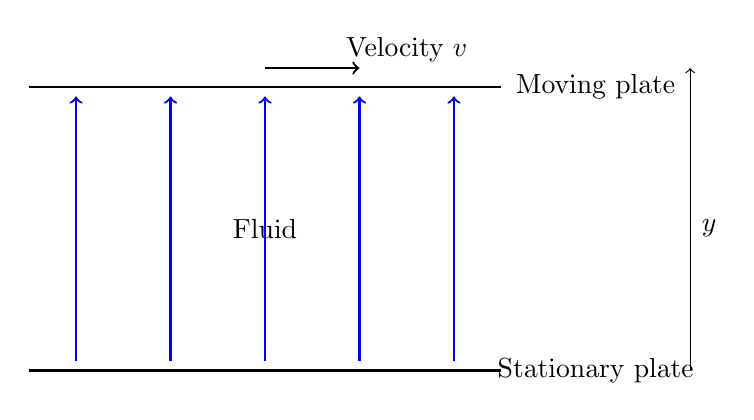
\begin{tikzpicture}[scale=1.2]

% Draw the stationary bottom plate
\draw[thick] (0,0) -- (5,0);
\node at (6, 0) {Stationary plate};

% Draw the top moving plate
\draw[thick] (0,3) -- (5,3);
\draw[->, thick] (2.5,3.2) -- (3.5,3.2);
\node at (4, 3.4) {Velocity $v$};
\node at (6, 3) {Moving plate};

% Draw the velocity gradient (linear)
\foreach \x in {0.5,1.5,2.5,3.5,4.5}
{
    \draw[->, blue, thick] (\x,0.1) -- (\x,2.9);
}

% Label axes
\draw[->] (7,0) -- (7,3.2);
\node at (7.2,1.5) {$y$};

% Add fluid label
\node at (2.5, 1.5) {Fluid};
\end{tikzpicture}
\caption{Fluid between two plates}\label{fig:fluid-plates(6)}
\end{figure}

The linear viscous force for this setup is given by 
\begin{gather}
    F = \mu A \dv{v}{y} \notag \\
    \intertext{Defining the stress, we get} \notag 
    \sigma = \frac{F}{A} = \mu \dv{v}{y} \tag{10.1.1}
\end{gather}
\\
The above definition however, is not generally true. This is because fluid flow can exist in all 3 dimensions. In this section, I would like to expand this to all dimensions and get a general form of the viscous force. Further, I would like to get an expression for the force density.

\subsection{Velocity Field}
The velocity in 3-D space has 3 components, each along one of the axes. Therefore, the velocity field is defined by:
\[
    \vec{v}(\vec{r}, t) = \begin{pmatrix}
        v_x(x(t), y(t), z(t), t) \\ v_y(x(t), y(t), z(t), t) \\ v_z(x(t), y(t), z(t), t)
    \end{pmatrix}
\]

\subsection{Stress}
Stress is defined as the ratio of the force to the area on which the force acts. (10.1.1) defines the stress along x axis. In this subsection, I would like to extend this idea to all 3 spatial dimensions. It is to be noted that the components of stress are coupled.

Consider a cubic fluid element\cite{stress_tensor} of sides $dx$, $dy$, and $dz$. 

\begin{figure}[H]
\centering
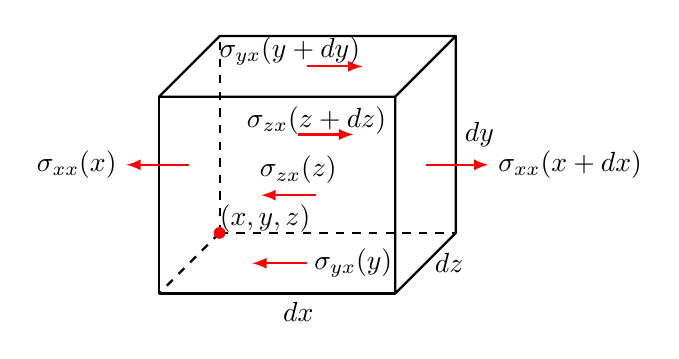
\begin{tikzpicture}[line join=round,>=latex]
    
        % Define cube origin and dimensions
        \coordinate (O) at (0,0,0);
        \coordinate (X) at (3,0,0);
        \coordinate (Y) at (0,2.5,0);
        \coordinate (Z) at (0,0,2);
        
        % Draw cube
        \draw[thick, dashed] (O) -- (X);
        \draw[thick, dashed] (O) -- (Y);
        \draw[thick, dashed] (O) -- (Z);
        \draw[thick] (X) -- ++(0,2.5,0) -- ++(0,0,2) -- ++(0,-2.5,0) -- cycle;
        \draw[thick] (Y) -- ++(3,0,0) -- ++(0,0,2) -- ++(-3,0,0) -- cycle;
        \draw[thick] (Z) -- ++(3,0,0) -- ++(0,2.5,0) -- ++(-3,0,0) -- cycle;
        
        % Node for center (x,y,z)
        \node at (0.5,0.1,-0.2) {$(x,y,z)$};
        \node at (0, 0, 0) [circle, fill=red, inner sep=1.5pt] {};
        
        % Stress vectors
        % Sigma_xx at left face
        \draw[->, thick, red] (0,1.25,1) -- ++(-0.8,0,0);
        \node[left] at (-0.8,1.25,1) {\(\sigma_{xx}(x)\)};
        
        % Sigma_xx at right face
        \draw[->, thick, red] (3,1.25,1) -- ++(0.8,0,0);
        \node[right] at (3.8,1.25,1) {\(\sigma_{xx}(x+dx)\)};
        
        % Tau_yx at bottom front
        \draw[->, thick, red] (1.5,0,1) -- ++(-0.7,0,0);
        \node[left] at (2.7,0,1) {\(\sigma_{yx}(y)\)};
        
        % Tau_yx at top front
        \draw[->, thick, red] (1.5,2.5,1) -- ++(0.7,0,0);
        \node[left] at (2.1,2.5,0.5) {\(\sigma_{yx}(y+dy)\)};
        
        % Tau_zx at back face
        \draw[->, thick, red] (1,1.25,0) -- ++(0.7,0,0);
        \node[below] at (1.5,2,0.7) {\(\sigma_{zx}(z+dz)\)};
        
        % Tau_zx at front face
        \draw[->, thick, red] (2,1.25,2) -- ++(-0.7,0,0);
        \node[above] at (1.5,1,1.3) {\(\sigma_{zx}(z)\)};
        
        % Axis labels
        \node at (1,-1,0) {$dx$};
        \node at (3.3,1.25,0) {$dy$};
        \node at (3.3,0,1.0) {$dz$};
    
    \end{tikzpicture}
\caption{Cubical fluid element}\label{fig:cubical-fluid-element(7)}
\end{figure}

In the above figure, \(\sigma_{xx}\) is the stress acting parallel to x axis on the area perpendicular to x axis.\ \(\sigma_{yx}\) is the stress acting parallel to x axis on the area perpendicular to y axis.\ \(\sigma_{zx}\) is the stress acting parallel to x axis on the area perpendicular to the z axis.

Let \(A_i\) denote the area perpendicular to the \(i\) axis. The force due to these stresses is given by:
\begin{align}
    F_x &= [\sigma_{xx} (x+dx) - \sigma_{xx}(x)]A_x \notag \\
        &\quad + [\sigma_{yx} (y+dy) - \sigma_{yx}(y)]A_y \notag \\
        &\quad + [\sigma_{zx} (z+dz) - \sigma_{zx}(z)]A_z \notag
\end{align}
Using the relation $F_x = \rho \dd{x} \dd{y} \dd{z} a_x$
\begin{align}
     \rho \dd{x} \dd{y} \dd{z} a_x &=  [\sigma_{xx} (x+dx) - \sigma_{xx}(x)]\dd{y} \dd{z} \notag \\
        &\quad + [\sigma_{yx} (y+dy) - \sigma_{yx}(y)]\dd{x} \dd{z} \notag \\
        &\quad + [\sigma_{zx} (z+dz) - \sigma_{zx}(z)]\dd{x} \dd{y} \notag
\end{align}
Dividing by the volume element \(\dd{x} \dd{y} \dd{z}\) on both sides, we get
\[
    \rho a_x = \frac{\sigma_{xx} (x+dx) - \sigma_{xx}(x)}{\dd{x}} + \frac{\sigma_{yx} (y+dy) - \sigma_{yx}(y)}{\dd{y}} + \frac{\sigma_{zx} (z+dz) - \sigma_{zx}(z)}{\dd{z}}
\]
Taking the limit $\dd{i} \to 0 \quad (i \in \{x, y, z\})$, the result simplifies to the following
\[
    \rho a_x = \pdv{\sigma_{xx}}{x} + \pdv{\sigma_{yx}}{y} + \pdv{\sigma_{zx}}{z} \tag{10.3.1a}
\]
Similarly
\begin{align}
    \rho a_y &= \pdv{\sigma_{xy}}{x} + \pdv{\sigma_{yy}}{y} + \pdv{\sigma_{zy}}{z} \tag{10.3.1b} \\
    \rho a_z &= \pdv{\sigma_{xz}}{x} + \pdv{\sigma_{yz}}{y} + \pdv{\sigma_{zz}}{z} \tag{10.3.1c}
\end{align}

Therefore
\begin{align}
    \rho \vec{a} &= \qty(\pdv{\sigma_{xx}}{x} + \pdv{\sigma_{yx}}{y} + \pdv{\sigma_{zx}}{z}) \hat{x} \notag \\
    &+ \qty(\pdv{\sigma_{xy}}{x} + \pdv{\sigma_{yy}}{y} + \pdv{\sigma_{zy}}{z}) \hat{y} \notag \\
    &+ \qty(\pdv{\sigma_{xz}}{x} + \pdv{\sigma_{yz}}{y} + \pdv{\sigma_{zz}}{z}) \hat{z} \notag
\end{align}

As can be seen, this result has a lot of information and can get confusing. Therefore, switching to matrices would be helpful.

Firstly, I define the viscous stress matrix, as:
\[
    \bm{S} = \begin{pmatrix}
        \sigma_{xx} & \sigma_{xy} & \sigma_{xz} \\ \sigma_{yx} & \sigma_{yy} & \sigma_{yz} \\ \sigma_{zx} & \sigma_{zy} & \sigma_{zz}
    \end{pmatrix}
\]
The divergence of the matrix is given by:
\[
    \nabla \cdot \bm{S} = \begin{pmatrix} \displaystyle
        \pdv{x} \\[1.5em] \displaystyle \pdv{y} \\[1.5em] \displaystyle \pdv{z}
    \end{pmatrix} \cdot \begin{pmatrix}
        \sigma_{xx} & \sigma_{xy} & \sigma_{xz} \\ \sigma_{yx} & \sigma_{yy} & \sigma_{yz} \\ \sigma_{zx} & \sigma_{zy} & \sigma_{zz}
    \end{pmatrix}
\]
Using $a \cdot b = a^T b$, we arrive at the following equation
\[
    \nabla \cdot \bm{S} = \begin{pmatrix} \displaystyle
        \pdv{\sigma_{xx}}{x} + \pdv{\sigma_{yx}}{y} + \pdv{\sigma_{zx}}{z} \\[1.5em] \displaystyle
        \pdv{\sigma_{xy}}{x} + \pdv{\sigma_{yy}}{y} + \pdv{\sigma_{zy}}{z} \\[1.5em] \displaystyle
        \pdv{\sigma_{xz}}{x} + \pdv{\sigma_{yz}}{y} + \pdv{\sigma_{zz}}{z}
    \end{pmatrix} \tag{10.3.2}
\]

Therefore
\[
    \vec{f} = \rho \vec{a} = \nabla \cdot \bm{S} \tag{10.3.3}
\]

\subsubsection{Newton's Law of viscosity}
From (10.3.2), we have:
\begin{gather}
    \dv{\vec{F}}{V} = \nabla \cdot \bm{S} \notag \\
    \implies \vec{F} = \int_V (\nabla \cdot \bm{S}) \dd{V} \notag \\
    \intertext{Using Gauss' Divergence theorem}
    \vec{F} = \int_A \bm{S} \cdot \dd{\vec{A}} \tag{10.3.1.1}
\end{gather}

Considering the situation in Fig. 6, \(\bm{S}\) must simplify to \(\mu \dv{v}{y}\). Therefore:
\[
    F = \mu A \dv{v}{y}
\]

\subsection{Stress in terms of velocity}
To write the equation of motion in fluids, it would be better if the viscous force density could be expressed in terms of the velocity or operators acting on it. From equation (10.1.1), it is known that the stress is directly proportional to the velocity gradient.

Initially and intuitively, I had assumed that
\[
    \sigma_{ij} = \mu \pdv{v_i}{j}
\]
However, intuition can be wrong, or in this case, incomplete. The correct form of the stress in terms of the velocity gradients (after referring to external sources~\cite{landau}) is given by:
\[
    \sigma_{ij} = \mu \qty(\pdv{v_i}{j} + \pdv{v_j}{i})
\]
The only explanation that I could come up with for this is as follows. Since $\sigma_{ij}$ refers to the stress acting to the area perpendicular to $i$ directed towards $j$. The change in velocity of the face perpendicular to $i$ will also have to be accounted for. Therefore
\[
    \sigma_{ij} = \sigma_{ji}
\]

Substituting the values of $i$ and $j$ accordingly in the viscous stress matrix, we arrive at:
\[
    \bm{S} = \mu \begin{pmatrix}
        \displaystyle 2 \pdv{v_x}{x} & \displaystyle \pdv{v_x}{y} + \pdv{v_y}{x} & \displaystyle \pdv{v_x}{z} + \pdv{v_z}{x} \\[1.5em]
        \displaystyle \pdv{v_y}{x} + \pdv{v_x}{y} &  \displaystyle 2 \pdv{v_y}{y} &  \displaystyle \pdv{v_y}{z} + \pdv{v_z}{y} \\[1.5em]
        \displaystyle \pdv{v_z}{x} + \pdv{v_x}{z} & \displaystyle \pdv{v_z}{y} + \pdv{v_y}{z} &  \displaystyle 2 \pdv{v_z}{z}
    \end{pmatrix}
\]

Given that the velocity field is:
\[
    \vec{v} = \begin{pmatrix}
        v_x \\ v_y \\ v_z
    \end{pmatrix}
\]

Define the gradient of the velocity field to be
\[
    \nabla \vec{v} = \begin{pmatrix}
        \nabla v_x & \nabla v_y & \nabla v_z
    \end{pmatrix}
    = \begin{pmatrix}
        \displaystyle \pdv{v_x}{x} & \displaystyle \pdv{v_y}{x} & \displaystyle \pdv{v_z}{x} \\[1.5em]
        \displaystyle \pdv{v_x}{y} & \displaystyle \pdv{v_y}{y} & \displaystyle \pdv{v_z}{y} \\[1.5em]
        \displaystyle \pdv{v_x}{z} & \displaystyle \pdv{v_y}{z} & \displaystyle \pdv{v_z}{z}
    \end{pmatrix} \notag \\
\]

Therefore
\begin{equation}
    \bm{S} = \mu (\nabla \vec{v} + {(\nabla \vec{v})}^T) \tag{10.5.1} \label{eq:stress_tensor}
\end{equation}

Now, consider the divergence of the viscous stress matrix
\begin{align}
    \nabla \cdot \bm{S} &= \nabla \cdot [\mu (\nabla \vec{v} + {(\nabla \vec{v})}^T)] \notag \\
    &= \mu (\nabla \cdot \nabla \vec{v} + \nabla \cdot {(\nabla \vec{v})}^T) \notag \\
    &= \mu (\nabla^2 \vec{v} + \nabla \cdot {(\nabla \vec{v})}^T) \notag
\end{align}

Note that
\begin{align*}
    \nabla \cdot {(\nabla \vec{v})}^T &= \begin{pmatrix} \displaystyle
        \pdv{}{x} \\[1.5em] \displaystyle \pdv{}{y} \\[1.5em] \displaystyle \pdv{}{z}
    \end{pmatrix} \cdot 
    \begin{pmatrix} \displaystyle
        \pdv{v_x}{x} & \displaystyle \pdv{v_x}{y} & \displaystyle \pdv{v_x}{z} \\[1.5em] \displaystyle
        \pdv{v_y}{x} & \displaystyle \pdv{v_y}{y} & \displaystyle \pdv{v_y}{z} \\[1.5em] \displaystyle
        \pdv{v_z}{z} & \displaystyle \pdv{v_z}{y} & \displaystyle \pdv{v_z}{z}
    \end{pmatrix} \notag \\\\
    &= \begin{pmatrix} \displaystyle
        \pdv[2]{v_x}{x} + \pdv{v_y}{y}{x} + \pdv{v_z}{z}{x} \\[1.5em] \displaystyle
        \pdv{v_x}{x}{y} + \pdv[2]{v_y}{y} + \pdv{v_z}{z}{y} \\[1.5em] \displaystyle
        \pdv{v_x}{x}{z} + \pdv{v_y}{y}{z} + \pdv[2]{v_z}{z}
    \end{pmatrix} \notag  \\\\
    &= \begin{pmatrix} \displaystyle
        \pdv[2]{v_x}{x} + \pdv{v_y}{x}{y} + \pdv{v_z}{x}{z} \\[1.5em] \displaystyle
        \pdv{v_x}{y}{x} + \pdv[2]{v_y}{y} + \pdv{v_z}{y}{z} \\[1.5em] \displaystyle
        \pdv{v_x}{z}{x} + \pdv{v_y}{z}{y} + \pdv[2]{v_z}{z}
    \end{pmatrix} \quad \text{(By Schwarz's Theorem)} \notag \\\\
    &= \begin{pmatrix} \displaystyle
        \pdv{}{x} \\[1.5em] \displaystyle \pdv{}{y} \\[1.5em] \displaystyle \pdv{}{z}
    \end{pmatrix} \qty(\pdv{v_x}{x} + \pdv{v_y}{y} + \pdv{v_z}{z}) \notag \\\\
    &= \nabla(\nabla \cdot \vec{v}) \notag
\end{align*}

Therefore,
\[
    \nabla \cdot \bm{S} = \mu(\nabla^2 \vec{v} + \nabla(\nabla \cdot \vec{v})) \tag{10.5.2}
\]
assuming incompressibility
\[
    \nabla \cdot \bm{S} = \mu \nabla^2 \vec{v} \tag{10.5.3}
\]

\subsection{The force equation including viscous force}
Letting go of the assumption that the force due to the pressure gradient is now zero, we arrive at a general force equation including the viscous force.
\[
    \rho \qty(\pdv{\vec{v}}{t} + \vec{v} \cdot \nabla \vec{v}) = -\nabla P + \nabla \cdot \bm{S} \tag{10.5.4}
\]
In the presence of external forces, we can define the force density as \(\vec{f}_{\text{ext}} = \dv{\vec{F}}{V}\)
Therefore
\begin{equation*}
    \rho \qty(\pdv{\vec{v}}{t} + \vec{v} \cdot \nabla \vec{v}) = -\nabla P + \nabla \cdot \bm{S} + \vec{f}_{\text{ext}} \tag{10.5.5}\label{eq:navier_stokes}
\end{equation*}

\subsection{Work done by the viscous force}
The viscous force does work. From experience, it should be obvious that the viscous force does negative (dissipative) work. The force is also non-conservative. This is because more heat is dissipated by the viscous force when the path is longer, which implies that the work done by this force is path dependent.
\\
It is known that 
\[
    w_{vis} = \int_\Gamma \vec{f}_{vis} \cdot \dd{\vec{r}}
\]

Where $w_{vis}$ denotes the work done by the viscous force per unit volume. Substituting $\vec{f} = \nabla \cdot \bm{S}$, we get
\[
    w_{vis} = \mu \int_\Gamma (\nabla^2 \vec{v} + \nabla(\nabla \cdot \vec{v})) \cdot \dd{\vec{r}}
\]
Considering the incompressible case, that is, $\nabla \cdot \vec{v} = 0$, then
\[
    w_{vis} = \mu \int_\Gamma \nabla^2 \vec{v} \cdot \dd{\vec{r}} 
\]

In order to solve this integral, a few assumptions will be made. We will be assuming that
\begin{enumerate}
    \item The fluid is viscous
    \item There is only steady and laminar flow
    \item The fluid is incompressible
\end{enumerate}

From the force equation (neglecting external forces), we have:
\[
    \rho \dv{\vec{v}}{t} = -\nabla P + \mu \nabla^2 \vec{v}
\]

In steady flow, the acceleration is zero. Therefore
\begin{gather}
    0 = -\nabla P + \mu \nabla^2 \vec{v} \notag \\
    \implies \mu \nabla^2 \vec{v} = \nabla P \notag
\end{gather}

Taking the line integral on both sides, we get:
\begin{align}
    \mu \int_\Gamma \nabla^2 \vec{v} \cdot \dd{\vec{r}} &= \int_\Gamma \nabla P \cdot \dd{\vec{r}} \notag \\
    &= \Delta P \quad \text{(By Gradient Theorem)} \notag
\end{align}

In real viscous flow, pressure usually drops along the flow, therefore $\Delta P < 0$. Hence, it can be concluded that:
\[
    w_{vis} = \mu \int_\Gamma \nabla^2 \vec{v} \cdot \dd{\vec{r}} = \Delta P < 0 \tag{10.6.1}
\]

\subsection{Thermodynamics of viscosity}
The first law of Thermodynamics in differential form is given by
\[
    \dd{U} = \delta Q + \delta W
\]

Where,
\begin{center}
    U = internal energy, Q = heat, W = work
\end{center}
Note that $\delta$ represents an inexact differential.

\subsubsection{Entropy of viscous flow}
I would like to get an expression for the entropy change due to viscous dissipation. For this, I will be using the relations
\[
    \delta Q = T\dd{S} \quad \text{and} \quad \delta W = -P\dd{V} + w_{vis} \dd{V}
\]

Rearranging for $\dd{S}$, we get
\[
    \dd{S} = \frac{1}{T} [\dd{U} + (P-w_{vis}) \dd{V}]
\]

Using $\dd{U} = nC_V \dd{T}$, assuming that the fluid is an ideal gas ($P=\frac{nRT}{V}$) and the viscosity coefficient is not dependent on temperature,
\[
    \Delta S = nC_V\int_{T_1}^{T_2} \frac{\dd{T}}{T} + nR \int_{V_1}^{V_2} \frac{\dd{V}}{V} - \int_{V_1}^{V_2} \frac{w_{vis}}{T} \dd{V}
\]
The first and second integrals are easy to evaluate. However the third integral requires a little effort. The result simplifies to
\[
    \Delta S = nC_V \ln(\frac{T_2}{T_1}) + nR \ln(\frac{V_2}{V_1}) - \int_{V_1}^{V_2} \frac{w_{vis}}{T} \dd{V}
\]
Writing the first 2 terms as the change in entropy due to the reversible process of the ideal gas and the third one as the change in entropy due to viscous effects, we have
\[
    \Delta S = \Delta S_{ideal} - \int_{V_1}^{V_2} \frac{w_{vis}}{T} \dd{V}
\]

Since the heat dissipated by the viscosity is due to the work. We can use the first law once again, which implies:
\[
    \delta Q_{vis} = - \delta W_{vis}
\]

From the Clausius identity,
\[
    \dd{S}_{vis} = \frac{\delta Q_{vis}}{T}
\]

Therefore, 
\begin{equation}
    \Delta S_{vis} = -\int_{V_1}^{V_2} \frac{w_{vis}}{T} \dd{V} \label{eq:viscous_entropy}
\end{equation}
Since the viscous work is negative, the effective change in entropy is thus increased by the heat dissipated by viscosity.

% \subsubsection{Energy dissipation}

\section{Other coordinate systems}
\subsection{Spherical coordinates}
The spherical coordinate system uses $r$, $\theta$, and $\varphi$
\begin{figure}[H]
    \centering
    \includegraphics[width=0.5\linewidth]{image.png}
\end{figure}

\subsubsection{Acceleration}
The velocity field is given by the following vector:
\[
    \vec{v} = \begin{pmatrix}
        v_r \\ v_\theta \\ v_\varphi
    \end{pmatrix}
\]
if $\vec{v} = \vec{v}(r(t), \theta (t), \varphi (t), t)$
\begin{align*}
    \dv{\vec{v}}{t} &= \pdv{\vec{v}}{t} + \pdv{\vec{v}}{r} \dv{r}{t} + \pdv{\vec{v}}{\theta} \dv{\theta}{t} + \pdv{\vec{v}}{\varphi} \dv{\varphi}{t}\\
    &= \pdv{\vec{v}}{t} + v_r \pdv{\vec{v}}{r} + \frac{v_\theta}{r} \pdv{\vec{v}}{\theta} + \frac{v_\varphi}{r \sin{\theta}} \pdv{\vec{v}}{\varphi}
\end{align*}
Therefore
\[
    \nabla \equiv \begin{pmatrix} \displaystyle
        \pdv{}{r} \\[1.5em] \displaystyle \frac{1}{r} \pdv{}{\theta} \\[1.5em] \displaystyle \frac{1}{r \sin{\theta}} \pdv{}{\varphi}
    \end{pmatrix}
\]
And
\[
    \dv{\vec{v}}{t} = \pdv{\vec{v}}{t} + (\vec{v} \cdot \nabla) \vec{v}
\]

\subsubsection{Pressure gradient}
The gradient of the pressure in spherical coordinates is given by
\[
    \nabla P = \pdv{P}{r} \hat{r} + \frac{1}{r} \pdv{P}{\theta} \hat{\theta} + \frac{1}{r \sin{\theta}} \pdv{P}{\varphi} \hat{\varphi}
\]

\subsubsection{Viscosity}
Since the unit vectors are not constant in the spherical coordinate system. The laplacian is different from expected. The vector laplacian in spherical coordinates is given by

\[
\nabla^2 \vec{v} =
\begin{pmatrix}
\displaystyle
\nabla^2 v_r 
- \frac{2 v_r}{r^2}
- \frac{2}{r^2 \sin\theta} \pdv{(v_\theta \sin\theta)}{\theta}
- \frac{2}{r^2 \sin\theta} \pdv{v_\varphi}{\varphi} \\[1.5em]

\displaystyle
\nabla^2 v_\theta 
- \frac{v_\theta}{r^2 \sin^2\theta}
+ \frac{2}{r^2} \pdv{v_r}{\theta}
- \frac{2 \cos\theta}{r^2 \sin^2\theta} \pdv{v_\varphi}{\varphi} \\[1.5em]

\displaystyle
\nabla^2 v_\varphi 
- \frac{v_\varphi}{r^2 \sin^2\theta}
+ \frac{2}{r^2 \sin\theta} \pdv{v_r}{\varphi}
+ \frac{2 \cos\theta}{r^2 \sin^2\theta} \pdv{v_\theta}{\varphi}
\end{pmatrix}
\]

This arises from applying the scalar laplacian to every component of the velocity vector, including the unit vectors.


\subsubsection{The force equation in spherical coordinates}
The force equation in spherical coordinates in its full form is given by:
\begin{gather*}
\rho \left(
    \pdv{\vec{v}}{t}
    + v_r \pdv{\vec{v}}{r}
    + \frac{v_\theta}{r} \pdv{\vec{v}}{\theta}
    + \frac{v_\varphi}{r \sin{\theta}} \pdv{\vec{v}}{\varphi}
\right)
=
- \left(
    \pdv{P}{r} \hat{r}
    + \frac{1}{r} \pdv{P}{\theta} \hat{\theta}
    + \frac{1}{r \sin{\theta}} \pdv{P}{\varphi} \hat{\varphi}
\right) \\
+ \mu
\begin{pmatrix}
\displaystyle
\nabla^2 v_r
- \frac{2 v_r}{r^2}
- \frac{2}{r^2 \sin\theta} \pdv{(v_\theta \sin\theta)}{\theta}
- \frac{2}{r^2 \sin\theta} \pdv{v_\varphi}{\varphi} \\[1.5em]
\displaystyle
\nabla^2 v_\theta
- \frac{v_\theta}{r^2 \sin^2\theta}
+ \frac{2}{r^2} \pdv{v_r}{\theta}
- \frac{2 \cos\theta}{r^2 \sin^2\theta} \pdv{v_\varphi}{\varphi} \\[1.5em]
\displaystyle
\nabla^2 v_\varphi
- \frac{v_\varphi}{r^2 \sin^2\theta}
+ \frac{2}{r^2 \sin\theta} \pdv{v_r}{\varphi}
+ \frac{2 \cos\theta}{r^2 \sin^2\theta} \pdv{v_\theta}{\varphi}
\end{pmatrix}
+ \vec{f}_{\text{ext}}
\end{gather*}


Compactly written, the equation is identical to the equation in Cartesian coordinates
\[
    \rho \dv{\vec{v}}{t} = -\nabla P + \mu \nabla^2 \vec{v} + \vec{f}_{\text{ext}}
\]

\subsection{Cylindrical coordinates}
The cylindrical coordinate system uses $r$, $\varphi$ and $z$.

\begin{figure}[H]
    \centering
    \includegraphics[width=0.5\linewidth]{image2.png}
\end{figure}

\subsubsection{Acceleration}
The velocity field is given by the following vector:
\[
    \vec{v} = \begin{pmatrix}
        v_r \\ v_\varphi \\ v_z
    \end{pmatrix}
\]
if $\vec{v} = \vec{v}(r(t), \varphi(t), z(t), t)$
\begin{align*}
    \dv{\vec{v}}{t} &= \pdv{\vec{v}}{t} + \pdv{\vec{v}}{r} \dv{r}{t} + \pdv{\vec{v}}{z} \dv{z}{t} \\
    &= \pdv{\vec{v}}{t} + v_r \pdv{\vec{v}}{r} + \frac{v_\varphi}{r} \pdv{\vec{v}}{\varphi} + v_z \pdv{\vec{v}}{z}
\end{align*}
Therefore
\[
    \nabla \equiv \begin{pmatrix} \displaystyle
        \pdv{}{r} \\[1.5em]  \displaystyle \frac{1}{r} \pdv{}{\varphi} \\[1.5em] \displaystyle \pdv{}{z}
    \end{pmatrix}
\]
And
\[
    \dv{\vec{v}}{t} = \pdv{\vec{v}}{t} + (\vec{v} \cdot \nabla) \vec{v}
\]

\subsubsection{Pressure gradient}
The gradient of the pressure in cylindrical coordinates is given by
\[
    \nabla P = \pdv{P}{r} \hat{r} + \frac{1}{r} \pdv{P}{\varphi} \hat{\varphi} + \pdv{P}{z} \hat{z}
\]


\subsubsection{Viscosity}
Similar to the spherical coordinates' unit vectors, the cylindrical coordinates have variable unit vectors. Therefore the laplacian in cylindrical coordinates is given by:
\[
\nabla^2 \vec{v} =
\begin{pmatrix}
\displaystyle
\nabla^2 v_r
- \frac{v_r}{r^2}
- \frac{2}{r^2} \pdv{v_\varphi}{\varphi} \\[1.5em]

\displaystyle
\nabla^2 v_\varphi
- \frac{v_\varphi}{r^2}
+ \frac{2}{r^2} \pdv{v_r}{\varphi} \\[1.5em]

\displaystyle
\nabla^2 v_z
\end{pmatrix}
\]


\subsubsection{The force equation in cylindrical coordinates}
The force equation in cylindrical coordinates in its full form is given by:
\begin{gather*}
    \rho \qty(\pdv{\vec{v}}{t} + v_r \pdv{\vec{v}}{r} + \frac{v_\varphi}{r} \pdv{\vec{v}}{\varphi} + v_z \pdv{\vec{v}}{z}) = -\qty(\pdv{P}{r} \hat{r} + \frac{1}{r} \pdv{P}{\varphi} \hat{\varphi} + \pdv{P}{z} \hat{z}) \\
    + 
    \mu 
    \begin{pmatrix}
    \displaystyle
    \nabla^2 v_r
    - \frac{v_r}{r^2}
    - \frac{2}{r^2} \pdv{v_\varphi}{\varphi} \\[1.5em]
    \displaystyle
    \nabla^2 v_\varphi
    - \frac{v_\varphi}{r^2}
    + \frac{2}{r^2} \pdv{v_r}{\varphi} \\[1.5em]
    \displaystyle
    \nabla^2 v_z
    \end{pmatrix} + \vec{f}_{\text{ext}}
\end{gather*}

Compactly written, the equation is identical to the equation in Cartesian coordinates
\[
    \rho \dv{\vec{v}}{t} = -\nabla P + \mu \nabla^2 \vec{v} + \vec{f}_{\text{ext}}
\]

\section{Solving for velocity}
For this part of the document, I referred to external sources\cite{landau} due to my limited knowledge of partial differential equations.

\subsection{Poiseuille Flow}
This is a special kind of flow. The figure is given below:

\begin{figure}[H]
\centering
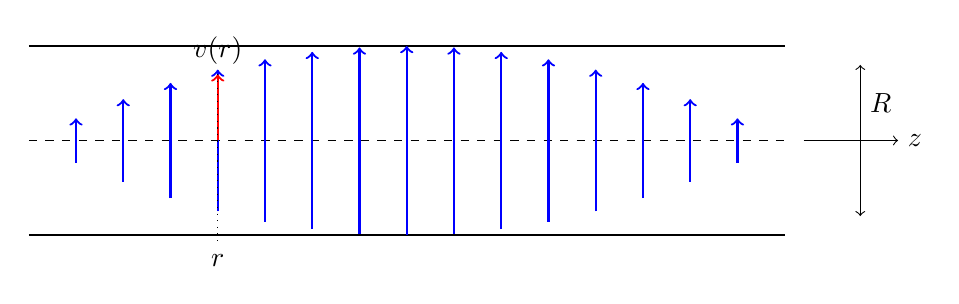
\begin{tikzpicture}[scale=1.2]

% Pipe boundaries
\draw[thick] (0,-1) -- (8,-1);
\draw[thick] (0,1) -- (8,1);
\draw[dashed] (0,0) -- (8,0);

% Velocity profile (parabolic)
\foreach \x in {0.5,1,...,7.5} {
  \pgfmathsetmacro{\len}{1 - ((\x - 4)^2)/16}
  \draw[->, blue, thick] (\x,-\len) -- (\x,\len);
}

% Axis and labels
\draw[->] (8.2,0) -- (9.2,0) node[right] {$z$};
\draw[<->] (8.8,0.8) -- (8.8,-0.8);
\node[right] at (8.8,0.4) {$R$};

% Velocity label
\draw[->, red, thick] (2,0) -- (2,0.7);
\node[above] at (2,0.7) {$v(r)$};
\draw[dotted] (2,0.7) -- (2,0);
\draw[dotted] (2,0) -- (2,-1.1);
\node[below] at (2,-1.1) {$r$};

\end{tikzpicture}
\caption{Poiseuille flow profile}\label{fig:posseuille-flow-profile(8)}
\end{figure}

The following assumptions are made
\begin{itemize}
    \item \textbf{Steady flow:} \(\displaystyle \pdv{\vec{v}}{t} = 0\)
    \item \textbf{Incompressible fluid:} \(\displaystyle \nabla \cdot \vec{v} = 0\)
    \item \textbf{Unidirectional flow:} \(\vec{v} = v_z(r)\, \hat{z}\), with \(v_r = v_\varphi = 0\)
    \item \textbf{Fully developed flow:} \(\displaystyle \pdv{v_z}{z} = 0\)
    \item \textbf{Axisymmetric:} \(\displaystyle \pdv{v_z}{\varphi} = 0\)
    \item \textbf{No external body forces:} \(\vec{f}_{\text{ext}} = 0\)
    \item \textbf{Constant pressure gradient:} \(\displaystyle \dv{P}{z} = \text{constant}\)
    \item \textbf{No-slip boundary condition:} \(v_z(R) = 0\)
\end{itemize}

The force equation subject to the above assumptions condenses to:
\begin{gather*}
    0 = -\dv{P}{z} + \frac{\mu}{r}\dv{}{r}\qty(r \dv{v_z}{r}) \\
    \implies \frac{\mu}{r} \qty(r \dv[2]{v_z}{r} + \dv{v_z}{r}) = \dv{P}{z} \\
    \implies \mu \dv[2]{v_z}{r} + \frac{\mu}{r} \dv{v_z}{r} - \dv{P}{z} = 0 \\
    \implies \dv[2]{v_z}{r} + \frac{1}{r} \dv{v_z}{r} - \frac{1}{\mu} \dv{P}{z} = 0 \\
    \intertext{Rewriting $\frac{1}{\mu} \dv{P}{z} = K$}
    \dv[2]{v_z}{r} + \frac{1}{r} \dv{v_z}{r} - K = 0
\end{gather*}

The general solution to this differential equation is
\[
    v_z(r) = \frac{K}{4} r^2 + C_1 \ln{r} + C_2
\]
\begin{itemize}
    \item $r=0$: $v_z$ is finite $\implies C_1 = 0$
    \item $r=R$: $v_z=0$ by the no slip condition $\implies C_2 = -\frac{K}{4} R^2$
\end{itemize}
Therefore
\[
    \vec{v}(r) = \frac{\Delta P}{4 \mu z} (r^2 - R^2) (\hat{z}) \tag{12.1.1}
\]

\subsection{Couette Flow}
This is the flow of a viscous fluid between two parallel plates where one of the plates is stationary and the other is moving with a constant velocity. There is also no pressure gradient present. The diagram is given below.

\begin{figure}[H]
    \centering
    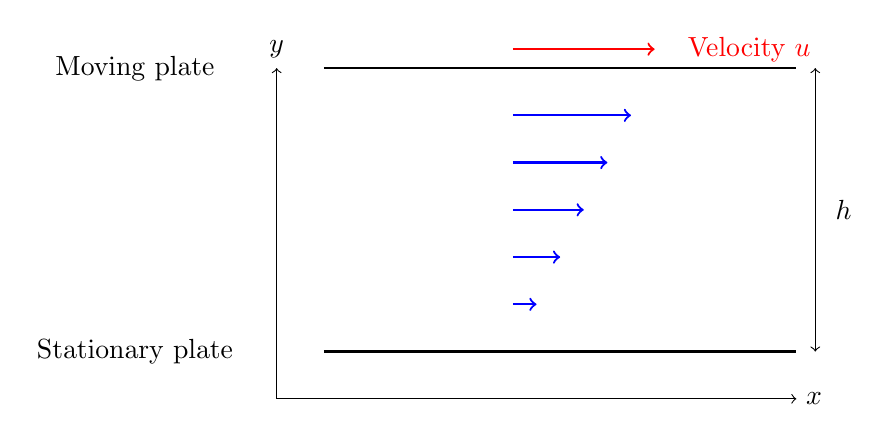
\begin{tikzpicture}[scale=1.2]
        % Plates
        \draw[thick] (0,0) -- (5,0); % bottom plate
        \draw[thick] (0,3) -- (5,3); % top plate

        % Labels
        \node at (-2, 0) {Stationary plate};
        \node at (-2, 3) {Moving plate};

        % Velocity profile
        \foreach \y in {0.5,1,1.5,2,2.5}
            \draw[->, blue, thick] (2,\y) -- ++(1.5*\y/3,0);

        % Distance label
        \draw[<->] (5.2,0) -- (5.2,3);
        \node at (5.5,1.5) {$h$};

        % Upper plate velocity vector
        \draw[->, red, thick] (2,3.2) -- ++(1.5,0);
        \node[red] at (4.5,3.2) {Velocity $u$};

        % Axes (optional)
        \draw[->] (-0.5,-0.5) -- ++(0,3.5) node[above] {$y$};
        \draw[->] (-0.5,-0.5) -- ++(5.5,-0.0) node[right] {$x$};
    \end{tikzpicture}
    \caption{Couette flow profile}\label{fig:couette-flow-profile(9)}
\end{figure}

The following assumptions are made
\begin{itemize}
    \item \textbf{Steady flow:} \(\displaystyle \pdv{\vec{v}}{t} = 0\)
    \item \textbf{Incompressible fluid:} \(\nabla \cdot \vec{v} = 0\)
    \item \textbf{Unidirectional flow:} \(\vec{v} = v_x(y) \hat{x}\)
    \item \textbf{No pressure gradient:} \(\displaystyle \pdv{P}{x} = 0\)
    \item \textbf{No body forces:} \(\vec{f}_{\text{ext}} = 0\)
    \item \textbf{Boundary condition:} flow is between two infinite parallel plates—top plate moves with velocity \(u\), bottom plate is stationary
\end{itemize}

The force equation subject to the above assumptions condenses to:
\begin{gather*}
    0 = \mu \dv[2]{v_x}{y} \hat{x} \\
    \intertext{Since this is true generally}
    \dv[2]{v_x}{y} = 0 \\
    \implies v_x(y) = C_1 y + C_2
\end{gather*}

\begin{itemize}
    \item $y=0$: $v_x = 0 \implies C_2 = 0$
    \item $y=h$: $v_x = u \implies C_1 = \frac{u}{h}$
\end{itemize}
Therefore
\[
    \vec{v}(y) = \frac{u}{h}y (\hat{x}) \tag{12.2.1}
\]

\subsection{Poiseuille-Couette Flow}
This is the flow of a viscous fluid between two parallel plates where one of the plates is stationary and the other is moving with a constant velocity. There is also a constant pressure gradient acting along the velocity, which drives the flow. The diagram is given below.

\begin{figure}[H]
    \centering
    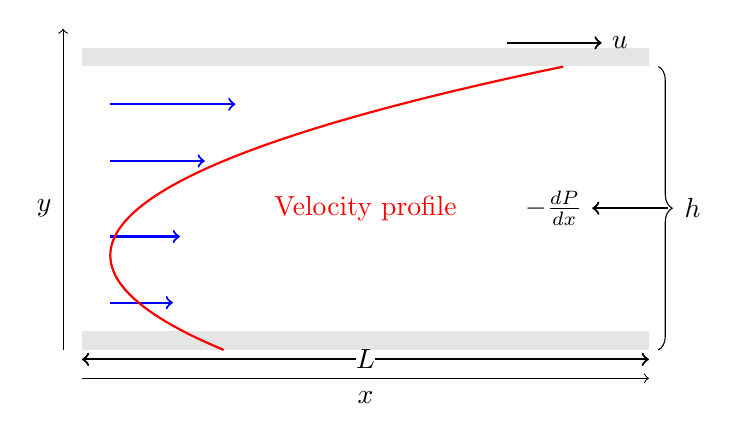
\begin{tikzpicture}[scale=1.2]

        % Geometry
        \def\h{3}  % Height between plates
        \def\L{6}  % Length of the channel

        % Plates
        \fill[gray!20] (0,0) rectangle (\L,0.2);         % Bottom plate
        \fill[gray!20] (0,\h) rectangle (\L,\h+0.2);      % Top plate

        % Flow direction arrows (velocity profile)
        \foreach \y in {0.5,1.2,2,2.6} {
            \pgfmathsetmacro{\vx}{0.5*\y*(\y - \h) + \y}  % Simplified velocity shape
            \draw[->, thick, blue] (0.3,\y) -- ++({0.7 + 0.3*\vx},0);
        }

        % Velocity profile curve (qualitative)
        \draw[thick, red, domain=0:\h, samples=100, smooth]
            plot({1.5 + 1.2*(\x*(\x - \h) + \x)}, {\x});

        % Axes labels
        \node at (-0.4, \h/2) {$y$};
        \draw[->] (-0.2, 0) -- (-0.2, \h+0.4);

        \node at (\L/2, -0.5) {$x$};
        \draw[->] (0, -0.3) -- (\L, -0.3);

        % Wall velocity
        \draw[->, thick] (4.5, \h+0.25) -- ++(1, 0) node[anchor=west] {$u$};

        % Pressure gradient
        \draw[->, thick] (\L+0.2, \h/2) -- ++(-0.8, 0) node[anchor=east] {$-\frac{dP}{dx}$};

        % Velocity profile label
        \node at (\L/2, \h/2) [red] {Velocity profile};

        % Length
        \node at (\L/2, -0.1) {$L$};
        \draw[<-, thick] (0, -0.1) -- (\L/2 - 0.1, -0.1);
        \draw[->, thick] (\L/2 + 0.1, -0.1) -- (\L, -0.1);

        % Bracket for h
        \draw[decorate,decoration={brace,amplitude=5pt, mirror}] (\L+0.1,0) -- (\L+0.1,\h) node[midway,right=6pt] {$h$};

    \end{tikzpicture}
    \caption{Poiseuille–Couette flow profile}\label{fig:poiseuille-couette-flow-profile(10)}
\end{figure}

The following assumptions are made
\begin{itemize}
    \item \textbf{Parallel Plates:} The flow occurs between two infinite, flat, parallel plates separated by a constant distance \( h \).
    
    \item \textbf{Steady Flow:} There is no time dependence; \( \partial \vec{v}/ \partial t = 0 \).
    
    \item \textbf{Fully Developed Flow:} The velocity profile does not change along the flow direction; \( \partial v_x / \partial x = 0 \).
    
    \item \textbf{Incompressible Fluid:} The fluid has constant density and satisfies \( \nabla \cdot \vec{v} = 0 \).
    
    \item \textbf{Newtonian Fluid:} The shear stress is proportional to the velocity gradient.
    
    \item \textbf{Constant Viscosity:} The dynamic viscosity \( \mu \) remains uniform throughout the fluid.
    
    \item \textbf{Unidirectional Flow:} Only the \( x \)-component of velocity is present, i.e., \( v_x = v_x(y) \), while \( v_y = v_z = 0 \).
    
    \item \textbf{No Slip at Walls:} The velocity at the walls matches that of the plates: \( v_x = 0 \) at the bottom, \( v_x = U \) at the top.
    
    \item \textbf{Constant Pressure Gradient:} A uniform pressure gradient \( -\frac{dP}{dx} \) drives the flow.
    
    \item \textbf{Negligible Body Forces:} $\vec{f}_{\text{ext}} = 0$.
\end{itemize}

The force equation subject to the above assumptions condenses to
\begin{gather*}
    0 = \qty[-\dv{P}{x} + \mu \dv[2]{v_x}{y}] (\hat{x})\\
    \implies \dv[2]{v_x}{y} = \frac{1}{\mu} \dv{P}{x} = K \quad \text{(Constant $\dv{P}{x}$)} \\
    \implies v_x(y) = \frac{K y^2}{2} + C_1 y + C_2
\end{gather*}

\begin{itemize}
    \item $y=0$: $v_x = 0 \implies C_2 = 0$
    \item $y=h$: $v_x = u \implies C_1 = \frac{u}{h} - \frac{K h}{2}$
\end{itemize}

Substituting $K = \frac{\Delta P}{\mu L}$, we get
\[
    \vec{v}(y) = \qty[\frac{\Delta P}{2 \mu L} y(y-h) + \frac{u}{h}y] (\hat{x}) \tag{12.3.1}
\]

\section{Frames of reference}

\subsection{Stationary frame}
In this description we fix a point in space and observe how the fluid flows past it. 
The velocity is treated as a field $\vec{v}(\vec{r},t)$. 
The material derivative of a quantity $\phi$ is
\[
    \qty{ \dv{}{t} }_{\text{total}} \equiv \pdv{}{t} + (\vec{v} \cdot \nabla).
\]

\subsection{Moving frame}
In this description we follow a particular fluid particle along its trajectory. 
The derivative is simply the ordinary time derivative:
\[
    \qty{ \dv{}{t} }_{\text{total}} \equiv \dv{}{t}.
\]



\section{Vortices}
As can be observed, vortices can be quantified using the velocity gradient in the perpendicular directions. That is, the gradient of \(v_x\) in $y$ and $z$ quantify the vorticity in the x direction, and so on.

\subsection{Vorticity}
Defining the vorticity by the following:
\[
    \vec{w} = \nabla \times \vec{v}
\]

Or, written more explicitly, the vorticity is given by:    
\begin{gather*}
    \begin{vmatrix}
            \hat{x} & \hat{y} & \hat{z} \\
            \partial_x & \partial_y & \partial_z \\
            v_x & v_y & v_z
    \end{vmatrix} \\
    \implies \vec{w} = \qty(\pdv{v_z}{y} - \pdv{v_y}{z}) \hat{x} + \qty(\pdv{v_x}{z} - \pdv{v_z}{x}) \hat{y} + \qty(\pdv{v_y}{x} - \pdv{v_x}{y}) \hat{z}
\end{gather*}
Thus, the curl of the velocity effectively quantifies how a component of the velocity profile changes in the directions perpendicular to it.

Similarly, in spherical coordinates, the vorticity is given by:
\begin{align*}
    \vec{w} &= \frac{1}{r \sin \theta} \qty(\pdv{(v_\varphi \sin \theta)}{\theta} - \pdv{v_\theta}{\varphi}) \hat{r} \\
    &+ \frac{1}{r} \qty(\frac{1}{\sin \theta} \pdv{v_r}{\varphi} - \pdv{(rv_\varphi)}{r}) \hat{\theta} \\
    &+ \frac{1}{r} \qty(\pdv{(r v_\theta)}{r} - \pdv{v_r}{\theta}) \hat{\varphi}
\end{align*}

Similarly, in cylindrical coordinates, the vorticity is given by:
\begin{align*}
    \vec{w} &= \qty(\frac{1}{r} \pdv{v_z}{\varphi} - \pdv{v_\varphi}{z}) \hat{r} \\
    &+ \qty(\pdv{v_r}{z} - \pdv{v_z}{r}) \hat{\varphi} \\
    &+ \frac{1}{r} \qty(\pdv{(r v_\varphi)}{r} - \pdv{v_r}{\varphi}) \hat{z}
\end{align*}

\subsection{Vorticity equation}
This subsection aims at arriving at a differential equation for the vorticity. The main aim to perform this is to eliminate the pressure gradient term from the equation. There are multiple vector identities in this section, for which I have used the internet.

Taking the curl on both the sides of the force equation
\begin{gather*}
    \nabla \times \qty(\rho \dv{\vec{v}}{t})= \nabla \times \qty(-\nabla P + \mu \nabla^2 \vec{v}) \\
    \implies (\nabla \rho) \times \dv{\vec{v}}{t} + \rho \qty(\nabla \times \dv{\vec{v}}{t}) = -\nabla \times \nabla P + \nabla \times \mu \nabla^2 \vec{v} \\
    \intertext{\text{Using the following identities:} $\qty(\nabla \times \dv{\vec{v}}{t} = \dv{(\nabla \times \vec{v})}{t})$  \text{and}  $\qty(\nabla \times \nabla P = 0)$ \text{, we get}}
    \nabla \rho \times \dv{\vec{v}}{t} + \rho \dv{\vec{w}}{t} = \nabla \times \mu \nabla^2 \vec{v} \\
    \intertext{\text{Once again assuming incompressibility, we get}}
    \rho \dv{\vec{w}}{t} = \nabla \times \mu \nabla^2 \vec{v} \\
    \implies \rho \dv{\vec{w}}{t} = \nabla \mu \times \nabla^2 \vec{v} + \mu (\nabla \times \nabla^2 \vec{v})
    \intertext{\text{Assuming that the viscosity coefficient is spatially invariant, we get}}
    \rho \dv{\vec{w}}{t} = \mu (\nabla \times \nabla^2 \vec{v})
    \intertext{\text{Using the vector identity: $\nabla^2 \vec{v} = \nabla(\nabla \cdot \vec{v}) - \nabla \times (\nabla \times \vec{v})$, we get}}
    \rho \dv{\vec{w}}{t} = \mu [\nabla \times \{\nabla(\nabla \cdot \vec{v}) - \nabla \times (\nabla \times \vec{v})\}] = -\mu (\nabla \times \nabla \times (\nabla \times \vec{v})) \\
    \implies \rho \dv{\vec{w}}{t} = - \mu(\nabla \times \nabla \times \vec{w})
    \intertext{This result implies that the vorticity dampens due to the viscosity.}
    \intertext{Using the vector identity: $\nabla \times \nabla \times \vec{w} = \nabla(\nabla \cdot \vec{w}) - \nabla^2 \vec{w}$}
    \implies \rho \dv{\vec{w}}{t} = -\mu [\nabla(\nabla \cdot \vec{w}) - \nabla^2 \vec{w}]
    \intertext{Substituting $\vec{w} = \nabla \times \vec{v}$, $\nabla(\nabla \cdot (\nabla \times \vec{v})) = 0$ (Divergence of the curl is 0)}
\end{gather*}
\begin{equation}
    \rho \dv{\vec{w}}{t} = \mu \nabla^2 \vec{w} \tag{14.2.1} \label{eq:vorticity1}
\end{equation}

In the above section, it was proven that the laplacian and the curl commute in the case when the density and coefficient of viscosity are constant.

\subsection{The total derivative of the vorticity}
To understand what the total derivative of the vorticity, the definition of the total derivative of velocity will be used. Taking the curl on both sides, we get:

\begin{align*}
    \nabla \times \qty(\dv{\vec{v}}{t}) &= \nabla \times \qty(\pdv{\vec{v}}{t} + (\vec{v} \cdot \nabla) \vec{v}) \\
    &= \pdv{(\nabla \times \vec{v})}{t} + \nabla \times (\vec{v} \cdot \nabla) \vec{v}
    \intertext{\text{Using the vector identity: }$\vec{v} \cdot \nabla \vec{v} = \frac{1}{2} \nabla |\vec{v}|^2 + (\nabla \times \vec{v}) \times \vec{v}$}
    &= \pdv{\vec{w}}{t} + \nabla \times \qty(\frac{1}{2} \nabla |\vec{v}|^2 + \vec{w} \times \vec{v}) \\
    &= \pdv{\vec{w}}{t} + \nabla \times (\vec{w} \times \vec{v})
    \intertext{Using the vector identity: $\nabla \times (\vec{w} \times \vec{v}) = \vec{w} (\nabla \cdot \vec{v}) - \vec{v} (\nabla \cdot \vec{w}) + (\vec{v} \cdot \nabla) \vec{w} - (\vec{w} \cdot \nabla) \vec{v}$}
    &= \pdv{\vec{w}}{t} + \vec{w} (\nabla \cdot \vec{v}) - \vec{v} (\nabla \cdot \vec{w}) + (\vec{v} \cdot \nabla) \vec{w} - (\vec{w} \cdot \nabla) \vec{v}
    \intertext{Once again, assuming incompressibility and the divergence of the vorticity being zero}
    &= \pdv{\vec{w}}{t} + (\vec{v} \cdot \nabla) \vec{w} - (\vec{w} \cdot \nabla) \vec{v} \tag{14.3.1}
\end{align*}

\subsection{Vorticity equation without external forces}
Substituting 13.3.1 in 13.2.1, we can get the complete expression for the vorticity equation

\[
    \rho \qty(\pdv{\vec{w}}{t} + (\vec{v} \cdot \nabla) \vec{w} - (\vec{w} \cdot \nabla) \vec{v}) = \mu \nabla^2 \vec{w}
\]

\subsection{Body forces}
If there were any external forces (represented by $\vec{f}$), performing all the operations above gives us the following result:
\[
    \rho \qty(\pdv{\vec{w}}{t} + (\vec{v} \cdot \nabla) \vec{w} - (\vec{w} \cdot \nabla) \vec{v}) = \mu \nabla^2 \vec{w} + \nabla \times \vec{f}
\]

\subsection{The final vorticity equation}
As we have assumed that the density is spatially invariant (or constant), we can perform further simplifications to the equation

\begin{gather*}
    \rho \qty(\pdv{\vec{w}}{t} + (\vec{v} \cdot \nabla) \vec{w} - (\vec{w} \cdot \nabla) \vec{v}) = \mu \nabla^2 \vec{w} + \nabla \times \vec{f} \\
    \implies \pdv{\vec{w}}{t} + (\vec{v} \cdot \nabla) \vec{w} - (\vec{w} \cdot \nabla) \vec{v} = \frac{\mu}{\rho} \nabla^2 \vec{w} + \frac{1}{\rho} (\nabla \times \vec{f}) \\
    \implies \pdv{\vec{w}}{t} + (\vec{v} \cdot \nabla) \vec{w} = (\vec{w} \cdot \nabla) \vec{v} + \frac{\mu}{\rho} \nabla^2 \vec{w} + \frac{1}{\rho} (\nabla \times \vec{f})
\end{gather*}

Finally, defining $\nu = \frac{\mu}{\rho}$, we get the final vorticity equation, which is:
\begin{equation}
    \pdv{\vec{w}}{t} + (\vec{v} \cdot \nabla) \vec{w} = (\vec{w} \cdot \nabla) \vec{v} + \nu \nabla^2 \vec{w} + \frac{1}{\rho} (\nabla \times \vec{f}) \tag{14.6.1} \label{eq:vorticity}
\end{equation}

\subsection{Physical interpretation of vorticity}
In 2-D, a positive vorticity implies that the velocity field is twisting in the anticlockwise direction and vice versa. However, in 3-D, the velocity field may twist, stretch and have more complex rotations along any of the axes. Nonetheless, the vectors still obey the right hand thumb rule. 

The term $(\vec{w} \cdot \nabla) \vec{v}$ refers to the vortex stretching\cite{landau}. It represents how $\vec{w}$ gets stretched/compressed by the velocity gradients in its own direction. The vorticity and velocity change in order to keep the angular momentum conserved.

The term $\nu \nabla^2 \vec{w}$ is similar to the laplacian term in the force equation. The vorticity flows from high to low regions, similar to diffusion.

\subsection{Solving for vorticity}
In this subsection, the vorticity will be solved for a certain velocity profile. The assumptions made are that the fluid is non-viscous and incompressible. 

Let the velocity vector be given by:
\[
    \vec{v} = \qty(-\frac{1}{2} \alpha x, -\frac{1}{2} \alpha y, \alpha z)
\]
Note that $\nabla \cdot \vec{v} = 0$

Finally, let the vorticity be subject to the initial condition:
\[
    \vec{w}(0) = w_0 \hat{z}
\]

Therefore, the vorticity equation condenses to the following:
\[
    \pdv{\vec{w}}{t} + (\vec{v} \cdot \nabla) \vec{w} = (\vec{w} \cdot \nabla) \vec{v}
\]

Let $\vec{r}$ be the trajectory vector $(\vec{r} = x\hat{x} + y\hat{y} + z\hat{z})$.
\begin{gather*}
    \dv{\vec{r}}{t} = \vec{v}(\vec{r}, t) = \qty(-\frac{1}{2} \alpha x, -\frac{1}{2} \alpha y, \alpha z)
    \intertext{Solving this yields the following solutions}
    x(t) = x_0 e^{-\frac{1}{2} \alpha t} \\
    y(t) = y_0 e^{-\frac{1}{2} \alpha t} \\
    z(t) = z_0 e^{\alpha t}
\end{gather*}

To solve for the vorticity along a path, the assumption $\vec{w}(t) = w_z(t) \hat{z}$ will be made. Lastly, as we are solving for vorticity along a path, the need to account for spatial variation is not required. Therefore, the second term on the left hand side of the vorticity equation vanishes.
\begin{gather*}
    \dv{\vec{w}}{t} = (\vec{w} \cdot \nabla) \vec{v} = w_z \pdv{\vec{v}}{z} = w_z \alpha \hat{z} \\
    \implies \dv{w_z}{t} = \alpha w_z \\
    \implies w_z(t) = w_0 e^{\alpha t} \\
    \implies \vec{w}(t) = w_0 e^{\alpha t} (\hat{z})
\end{gather*}

This result implies that the vorticity grows exponentially through the trajectory. This implies that vorticity can change even without viscosity and just by the existence of a velocity gradient. Therefore, velocity gradients cause vorticity.

\section{The field derivative}
The total derivative of a field vector always appears to appear in the form:
\[
    \pdv{}{t} + (\vec{v} \cdot \nabla)
\]
which implies that the frame of reference appears to move along with the fluid. Therefore, define the field derivative as follows:

\renewcommand{\fdv}[1]{%
  \if\relax\detokenize{#1}\relax
    \frac{\mathrm{D}}{\mathrm{D}t}
  \else
    \frac{\mathrm{D}#1}{\mathrm{D}t}
  \fi
}


\[
\boxed{
    \fdv{} \equiv \pdv{}{t} + (\vec{v} \cdot \nabla)
}
\]

The operator \(d_f\) combines the \textit{local rate of change} of the field at a fixed point in space and the \textit{convective change} due to fluid motion:

\[
    \fdv{\vec{A}(\vec{r}, t)} = \pdv{\vec{A}}{t} + (\vec{v}(\vec{r}, t) \cdot \nabla) \vec{A}(\vec{r}, t).
\]

\textbf{Interpretation:} \(D \vec{A}\) measures how the field \(\vec{A}\) changes \textit{as experienced by a fluid parcel moving with the flow}.



\section{Angular momentum in fluids}
Angular momentum is defined by the formula: $\vec{L} = \vec{r} \times \vec{p}$. Where $\vec{p}$ and $\vec{r}$ refer to the momentum and the position vectors. 

\subsection{Angular momentum density}
The common approach of getting expressions in terms of their densities applies to angular momentum as well. Let $\vec{l}$ define the angular momentum density.

\[
    \vec{l} = \vec{r} \times \rho \vec{v}
\]

To make sense of the terms in different reference frames, the description is given below.
\begin{enumerate}
    \item \textbf{Moving frame} \begin{itemize}
        \item $\vec{v}$: Velocity field
        \item $\vec{r}$: Position of the fluid parcel
    \end{itemize}

    \item \textbf{Static frame} \begin{itemize}
        \item $\vec{v}$: Velocity of the fluid at the frame of reference
        \item $\vec{r}$: Position of the frame of reference
    \end{itemize}
\end{enumerate}


\subsection{Angular momentum density time evolution}
In this subsection, the aim is to understand how the angular momentum density varies with time. So, the field derivative with respect to time will be taken.

\begin{align*}
    \fdv{\vec{l}} &= \fdv{(\vec{r} \times \rho\vec{v})} = \fdv{\vec{r}} \times \rho\vec{v} + \vec{r} \times \fdv{(\rho\vec{v})} \\
    &= \vec{v} \times \rho\vec{v} + \vec{r} \times \rho \fdv{\vec{v}}\\
    &= \vec{r} \times \rho \fdv{\vec{v}} \quad (\vec{v} \times \vec{v} = \vec{0}) \\
    &= \vec{r} \times \qty(-\nabla P + \nabla \cdot \bm{S}) \quad \text{(Force equation)} \tag{16.2.1}
\end{align*}

Therefore, the change in angular momentum density with time is equal to the torque density.

The torque density is given by:
\begin{gather*}
    \vec{\tau} = \vec{r} \times \vec{f} \\
    \implies \vec{\tau} = \vec{r} \times \rho \fdv{\vec{v}}\\
    \implies \vec{\tau} = \fdv{\vec{l}} \tag{16.2.2}
\end{gather*}

Further, since the fluid is assumed to be incompressible (i.e., constant $\rho$), we can move $\rho$ outside the derivative. Thus, we can write:
\[
    \vec{r} \times \left( \frac{\partial \vec{v}}{\partial t} + (\vec{v} \cdot \nabla)\vec{v} \right)
    = \left( \frac{\partial}{\partial t} + \vec{v} \cdot \nabla \right)(\vec{r} \times \vec{v})
\]

To see this explicitly:
\begin{gather*}
    \left( \frac{\partial}{\partial t} + \vec{v} \cdot \nabla \right)(\vec{r} \times \vec{v})
    = \left( \frac{\partial \vec{r}}{\partial t} + (\vec{v} \cdot \nabla)\vec{r} \right) \times \vec{v}
    + \vec{r} \times \left( \frac{\partial \vec{v}}{\partial t} + (\vec{v} \cdot \nabla)\vec{v} \right) \\
    = \vec{v} \times \vec{v} + \vec{r} \times \left( \frac{\partial \vec{v}}{\partial t} + (\vec{v} \cdot \nabla)\vec{v} \right)
    = \vec{r} \times \left( \frac{\partial \vec{v}}{\partial t} + (\vec{v} \cdot \nabla)\vec{v} \right)
\end{gather*}
since $\vec{v} \times \vec{v} = \vec{0}$.

\subsection{Conservation of angular momentum}
Similar to the linear momentum conservation equation, the angular momentum must be conserved. Therefore, the form of the equation is given by the following
\[
    \pdv{\vec{l}}{t} + \nabla \cdot (\text{Angular momentum flux}) = \vec{\tau}
\]
Which implies that if the angular momentum is varying with time and is not compensated by the flux, there will be an effective torque, as expected. The form of the angular momentum flux matrix is the angular version of that of the linear momentum flux matrix.

Therefore, the angular momentum conservation equation takes the following form:
\begin{equation}
    \pdv{(\vec{r} \times \rho \vec{v})}{t} + \nabla \cdot (\vec{r} \times \bm{M}) = \vec{\tau} \tag{16.3.1} \label{eq:angpflux}
\end{equation}
Where, $\bm{M}$ is the momentum flux matrix.

The cross product between a vector and a matrix is given by the following. If $\bm{M}$ is given by the following
\[
    \bm{M} = \begin{bmatrix}
        \vec{T}_1 & \vec{T}_2 & \vec{T}_3
    \end{bmatrix}
\]
\[
    \vec{r} \times \bm{M} = \begin{bmatrix}
        \vec{r} \times \vec{T}_1 & \vec{r} \times \vec{T}_2 & \vec{r} \times \vec{T}_3
    \end{bmatrix}
\]


\subsection{Angular velocity}
In classical mechanics, the relation between velocity and angular velocity is given by the following relation
\[
    \vec{v} = \vec{\omega} \times \vec{r}
\]
In this subsection, I aim to get an expression for $\vec{\omega}$ in terms of $\vec{v}$ and operators on it. Note that the dimensions of angular velocity and that of vorticity are the same, which suggests that there might be relation between the two. It also helps to know that the angular velocity vector points in the axis of rotation. Vorticity, being the curl of the velocity field, thus points in the same direction as that of the angular velocity. Therefore,
\[
    \vec{\omega} = k(\nabla \times \vec{v}) \quad \text{(k is a real number)}
\]

Consider a solid body rotation, where all the fluid particles rotate together around an axis. Therefore, the angular velocity is constant. Therefore
\begin{gather*}
    \vec{\omega} = \omega_z \hat{z} \\
    \vec{r} = x\hat{x} + y\hat{y} + z \hat{z} \\
    \vec{v} = \vec{\omega} \times \vec{r} = \omega_z(x\hat{y} - y \hat{x})
\end{gather*}

Computing the curl of the velocity field, we get
\begin{gather*}
    \vec{w} = \nabla \times \vec{v} \\
    \implies \vec{w} = \begin{vmatrix}
            \hat{x} & \hat{y} & \hat{z} \\
            \partial_x & \partial_y & \partial_z \\
            -\omega_z y & \omega_z x & 0
    \end{vmatrix} \\
    \implies w_x = \pdv{(0)}{y} - \pdv{(\omega_z x)}{z} = 0 \\
    \And w_y = -\pdv{(0)}{x} - \pdv{(\omega_z y)}{z} = 0 \\
    \And w_z = \pdv{(\omega_z x)}{x} + \pdv{(\omega_z y)}{y} = 2 \omega_z \\
    \implies \vec{\omega} = \frac{1}{2} (\nabla \times \vec{v}) \tag{16.4.1}
\end{gather*}

\section{Cooling in my hostel room}

Consider the setup where a room is being cooled by the following mechanism. A fan is placed at the door facing outwards. The fan blows air out of the room, which causes a low pressure region inside the room. Therefore, air from outside rushes in through the windows to equalize the pressure difference. Let the window be placed at $x = 0$ and the door be placed at $x = L$. 

The following observations were made: 
\begin{itemize}
    \item The flow of air from the windows is mostly horizontal. Therefore, the velocity profile is along the $x$ direction. By this assumption, if a cross section (passing through the door and the window) was to be examined, the velocity profile is only along the $x$ direction.
    \item The velocity profile is mostly uniform across the cross section of the window. Therefore, $v_x$ is not varying with $y$ or $z$. Thus, $\pdv{v_x}{y} = 0$ and $\pdv{v_x}{z} = 0$.
    \item At 7 PM, the temperature outside is around $27^\circ$C and the temperature inside is around $30^\circ$C before the fan is turned on.
    \item It takes around 2 to 3 minutes for the room to cool down.
\end{itemize}


The following assumptions are made:
\begin{itemize}
    \item The flow is incompressible.
    \item The flow is laminar.
    \item The flow is steady.
    \item The pressure gradient along $x$ is constant.
\end{itemize}

Let the pressure field be given by:
\[
    p(x) = p_0 + \frac{p_L - p_0}{L} x
\]

The force balance equation thus condenses to:
\[
    0 = -\dv{p}{x} + \mu \dv[2]{v_x}{x}
\]

Integrating twice, we get:
\[
v_x(x) = \frac{1}{2 \mu} \frac{p_L - p_0}{L} x^2 + A x + B
\]

Applying the boundary conditions:
\begin{gather*}
    v_x(0) = v_{\text{in}} \\
    v_x(L) = v_{\text{out}}
\end{gather*}

We get the following expressions for the constants:
\begin{align*}
    B &= v_{\text{in}} \\
    A &= \frac{v_{\text{out}} - v_{\text{in}}}{L} - \frac{p_L - p_0}{2\mu}
\end{align*}

Therefore, the velocity profile is given by:
\[
    v_x(x) = \frac{1}{2 \mu} \frac{p_L - p_0}{L} x^2 + \left( \frac{v_{\text{out}} - v_{\text{in}}}{L} - \frac{p_L - p_0}{2\mu} \right) x + v_{\text{in}}
\]

If the Reynolds number is very low (i.e., the flow is laminar and viscous forces dominate), the quadratic term is negligible compared to the linear term. Therefore, the velocity profile can be approximated as linear:
\[
    v_x(x) \approx v_{\text{in}} + \frac{v_{\text{out}} - v_{\text{in}}}{L} x
\]

Next, we calculate the volumetric flow rate. The volumetric flow rate is given by:
\[
    Q(x) = \iint v_x(x) \, \dd{A} = A \cdot v_x(x)
\]
where $A$ is the cross-sectional area of the window or door.

Therefore, the air flowing in through the window per second is:
\[
    Q(0) = A_{\text{in}} v_{\text{in}}
\]
and the air flowing out through the door per second is:
\[
    Q(L) = A_{\text{out}} v_{\text{out}}
\]

Since the flow is incompressible and steady, the volumetric flow rate must be conserved:
\begin{gather*}
    Q(0) = Q(L) \\
    \implies A_{\text{in}} v_{\text{in}} = A_{\text{out}} v_{\text{out}} \\
    \implies v_{\text{in}} = \frac{A_{\text{out}}}{A_{\text{in}}} v_{\text{out}}
\end{gather*}
After measuring, the area of the window is around 0.4 m² and the area of the fan's cross section is around 0.3 m². Therefore, $v_{\text{in}} = 0.75 v_{\text{out}}$.  

\subsection{Case 1: Normal fan speed}
Assuming the room has a volume of 60~m$^3$, the mass of air is:
\[
    m = \rho V = 1.15 \times 60 \approx 69~\mathrm{kg}
\]

The time required to cool the room is then:
\[
    t = \frac{m c_v \Delta T}{\dot{q}} = \frac{69 \times 718 \times 3}{372} \approx 400~\text{seconds} \approx 6.7~\text{minutes}
\]

\subsection{Case 2: Maximum fan speed}
If the fan is run at maximum speed $v_{\rm out} = 2.5~\mathrm{m/s}$, then $v_{\rm in} = 0.75 \times 2.5 = 1.875~\mathrm{m/s}$.

The cooling power becomes:
\[
    \dot{q} = \rho c_v A_{\rm in} v_{\rm in} \Delta T = 1.15 \times 718 \times 0.4 \times 1.875 \times 3 \approx 1856~\mathrm{W}
\]

The cooling time reduces to:
\[
    t = \frac{m c_v \Delta T}{\dot{q}} = \frac{69 \times 718 \times 3}{1856} \approx 80~\mathrm{seconds} \approx 1.3~\text{minutes}
\]

This shows that increasing the fan speed drastically reduces the time required to cool the room. Actual times may be slightly longer due to heat gain from humans, electrical appliances, walls, furniture, and imperfect mixing.

\section{Turbulence}
Turbulence is a chaotic state of fluid motion. It is flow which is `not' laminar. There is no actual definition of turbulence that I could think of. However, it is characterised by irregularity, diffusivity, high Reynolds number, three-dimensional vorticity fluctuations, and dissipation. The natural question to ask would be: When do laminar solutions of the force equation become unstable and chaotic?. Qualitatively, these solutions exhibit fluctuations over many length scales and are no longer smooth and predictable.

\subsection{Velocity decomposition}
Let $\vec{v}(\vec{r}, t)$ be a velocity field. It would make sense to split the velocity field into a mean and fluctuating part. Since the mean part is steady, it would not vary with time. Therefore,
\[
\vec{v}(\vec{r}, t) = \vec{V}(\vec{r}) + \vec{v'}(\vec{r}, t) \tag{18.1.1}
\]
Where, $\vec{V}(\vec{r})$ is the mean velocity field and $\vec{v'}(\vec{r}, t)$ is the fluctuating part of the velocity field. The mean velocity field is defined as:
\[
\vec{V}(\vec{r}) = \frac{\int \vec{v}(\vec{r}, t) \dd{t}}{\int \dd{t}}
\]
However, this indefinite integral makes no sense in a physical situation. Let $T$ be the time over which the average is being taken. Therefore
\[
\vec{V}(\vec{r}) = \frac{\int_{0}^{T} \vec{v}(\vec{r}, t) \dd{t}}{\int_{0}^{T} \dd{t}} = \frac{1}{T} \int_{0}^{T} \vec{v}(\vec{r}, t) \dd{t}
\]
Since, the steady state is being observed, it would make sense to take the limit to infinity. Therefore
\[
\vec{V}(\vec{r}) = \lim_{T \to \infty} \frac{1}{T} \int_{0}^{T} \vec{v}(\vec{r}, t) \dd{t}
\]

Furthermore, this is a valid decomposition if
\[
\lim_{T \to \infty} \frac{1}{T} \int_{0}^{T} \vec{v'}(\vec{r}, t) \dd{t} = 0
\]

Intuitively, if the fluctuations are very low, the velocity field would be very stable with time. Substituting the above expression in the force equation, we get

\[
\rho\, \fdv{\vec{v}} = - \nabla P + \mu \nabla^2 \vec{v}
\]

\[
\rho\, \fdv{(\vec{V} + \vec{v'})} = - \nabla P + \mu \nabla^2 (\vec{V} + \vec{v'})
\]

Since the average part is time invariant, it will only vary spatially in the field derivative:

\[
\pdv{\vec{V}}{t} = 0
\]

\[
\rho \left( \pdv{\vec{v'}}{t} + (\vec{V} + \vec{v'}) \cdot \nabla (\vec{V} + \vec{v'}) \right)
= -\nabla P + \mu \nabla^2 (\vec{V} + \vec{v'})
\]

For simplicity, let the density be of unit magnitude, which also implies that $\nu = \mu$:

\[
\pdv{\vec{v'}}{t} + (\vec{V} + \vec{v'}) \cdot \nabla (\vec{V} + \vec{v'})
= -\nabla P + \nu \nabla^2 (\vec{V} + \vec{v'})
\]

Since the gradient/laplacian is linear:

\[
\pdv{\vec{v'}}{t} + (\vec{V} + \vec{v'}) \cdot \nabla \vec{V} + (\vec{V} + \vec{v'}) \cdot \nabla \vec{v'}
= -\nabla P + \nu (\nabla^2 \vec{V} + \nabla^2 \vec{v'})
\]

As the dot product is distributive over addition:

\[
\pdv{\vec{v'}}{t} + \vec{V} \cdot \nabla \vec{V} + \vec{v'} \cdot \nabla \vec{V}
+ \vec{V} \cdot \nabla \vec{v'} + \vec{v'} \cdot \nabla \vec{v'}
= -\nabla P + \nu (\nabla^2 \vec{V} + \nabla^2 \vec{v'})
\]

\[
\fdv{\vec{v'}} = - \nabla P + \nu \nabla^2 \vec{v'} + \nu \nabla^2 \vec{V}
- (\vec{V} \cdot \nabla \vec{V} + \vec{v'} \cdot \nabla \vec{V}) \tag{18.1.2}
\]

Now, analysing the field derivative of the full velocity field, we get

\[
\fdv{\vec{v}} = \fdv{\vec{V}} + \fdv{\vec{v'}} + \vec{v'} \cdot \nabla \vec{V} \tag{18.1.3}
\]

\[
\fdv{\vec{v}} = (\vec{V} + \vec{v'}) \cdot \nabla \vec{V} - \nabla P
+ \nu \nabla^2 \vec{v'} + \nu \nabla^2 \vec{V}
- (\vec{V} \cdot \nabla \vec{V} + \vec{v'} \cdot \nabla \vec{V})
+ \vec{v'} \cdot \nabla \vec{V}
\]

\[
\fdv{\vec{v}} = -\nabla P + \nu \nabla^2 \vec{v}
\]

Therefore, the result for the field derivative of the fluctuation field is valid.

\subsection{Pressure decomposition}
It would make sense to decompose the pressure part as well. Or else, there would be no velocity field fluctuations. Therefore, define
\[
P(\vec{r}, t) = \bar{P}(\vec{r}) + P'(\vec{r}, t)
\]
where
\[
\bar{P} = \lim_{T \to \infty} \frac{1}{T} \int_{0}^{T} P \dd{t}
\]
Therefore, taking the gradients on both sides, we get
\[
\nabla P(\vec{r}, t) = \nabla \bar{P}(\vec{r}) + \nabla P'(\vec{r}, t) \tag{18.2.1}
\]

\subsection{Separating mean and fluctuating flows}
Let $\langle \rangle$ denote the time average function, that is,
\[
\langle \vec{v} \rangle = \lim_{T \to \infty} \frac{1}{T} \int_{0}^{T} \vec{v} \dd{t}
\]

Before doing any of the calculations, it would help to obtain a few general results with the time average function. 

Let $\vec{a}$ and $\vec{b}$ be any two vectors. We would like to find the time average of vector product $\vec{a} \cdot \nabla \vec{b}$
\begin{align*}
\langle \vec{a} \cdot \nabla \vec{b} \rangle &= \lim_{T \to \infty} \frac{1}{T} \int_{0}^{T} (\vec{a} \cdot \nabla \vec{b}) \dd{t} \\
&= \lim_{T \to \infty} \frac{1}{T} \int_{0}^{T} \qty(\sum_{i = x, y, z} a_i \pdv{\vec{b}}{i}) \dd{t} \\
&= \lim_{T \to \infty} \frac{1}{T} \sum_{i = x, y, z} \qty(\int_{0}^{T} a_i \pdv{\vec{b}}{i} \dd{t}) \\
&= \sum_{i=x, y, z} {(\langle \vec{a} \cdot \nabla \vec{b} \rangle)}_i 
\end{align*}
where
\[
{(\langle \vec{a} \cdot \nabla \vec{b} \rangle)}_i = \lim_{T \to \infty} \frac{1}{T} \int_{0}^{T} a_i \pdv{\vec{b}}{i} \dd{t}
\]

Let $a$ be any time averaged vector which represents a steady state, therefore, is invariant with time. It can be easily verified that
\[
\langle \vec{a} \rangle = \vec{a}
\]

As found, the mean and the fluctations comprise the entire velocity field. Taking the time average of the field derivative of the velocity field, we get
\[
\langle \fdv{\vec{v}} \rangle = \langle \pdv{\vec{v'}}{t} \rangle + \langle \vec{V} \cdot \nabla \vec{V} \rangle + \langle \vec{V} \cdot \nabla \vec{v'} \rangle + \langle \vec{v'} \cdot \nabla \vec{V} \rangle + \langle \vec{v'} \cdot \nabla \vec{v'} \rangle
\]

As $\vec{v'}$ is constructed in such a way that it's time average is zero. The above expression, from the properties of the time average funciton condenses to
\[
\langle \fdv{\vec{v}} \rangle = \vec{V} \cdot \nabla \vec{V} + \langle \vec{v'} \cdot \nabla \vec{v'} \rangle \tag{18.3.1}
\]

Note that
\[
\langle \fdv{\vec{v'}} \rangle = \langle \pdv{\vec{v'}}{t} \rangle + \langle (\vec{V} + \vec{v'}) \cdot \nabla \vec{v'} \rangle = \langle \vec{v'} \cdot \nabla \vec{v'} \rangle
\]

From (18.1.2), we have
\[
\fdv{\vec{v'}} = - \nabla \bar{P} - \nabla P' + \nu \nabla^2 \vec{v'} + \nu \nabla^2 \vec{V} - \vec{V} \cdot \nabla \vec{V} - \vec{v'} \cdot \nabla \vec{V}
\]
Applying $\langle \rangle$ on both sides of the equation, we get
\[
\langle \fdv{\vec{v'}} \rangle = -\nabla \bar{P} + \nu \nabla^2 \vec{V} - \vec{V} \cdot \nabla \vec{V}
\]
Note that these results look familiar to the momentum flux matrix terms. However, it will be dealt with a little later.

Finally, we have
\[
\langle \fdv{\vec{v}} \rangle = -\nabla \bar{P} + \nu \nabla^2 \vec{V} \tag{18.3.2}
\]

To verify this, we can use the fact that the whole field is a sum of the average and the fluctuating parts. Therefore from (18.1.1) and (18.2.1), we have
\[
\fdv{\vec{v}} = (-\nabla \bar{P} + \nu \nabla^2 \vec{V}) + (-\nabla P' + \nu \nabla^2 \vec{v'})
\]

Applying $\langle \rangle$ on both sides of the above equation, we get
\[
\langle \fdv{\vec{v}} \rangle = \langle -\nabla \bar{P} + \nu \nabla^2 \vec{V} \rangle + \langle -\nabla P' + \nu \nabla^2 \vec{v'} \rangle
\]
Once again, from the properties of $\langle \rangle$, the above equation finally condenses to the following
\[
\langle \fdv{\vec{v}} \rangle = -\nabla \bar{P} + \nu \nabla^2 \vec{V}
\]

Which is exactly what we calculated. Therefore, the result is correct.

\subsection{Turbulence stress matrix}
From (18.3.1), we have the result
\[
\langle \fdv{\vec{v}} \rangle = -\nabla \bar{P} + \langle \vec{v'} \cdot \nabla \vec{v'} \rangle
\]
Note that the first term is a steady state pressure gradient term and the second one is a fluctuating stress term. I would like to define the turbulence stress matrix as
\[
\nabla \cdot \bm{T} = \langle \vec{v'} \cdot \nabla \vec{v'} \rangle
\]
Following arguments similar to those in section 9.3 (Conservation of momentum), we arrive at the following
\[
\bm{T} = \langle \vec{v'} \vec{v'}^T \rangle \tag{18.4.1}
\]

I would also like to define a `Total Turbulence Matrix', which also accounts for the pressure term in the equation. Therefore, defining the matrix as $\bm{\kappa}$, we have
\[
\nabla \cdot \bm{\kappa} = -\nabla \bar{P} + \langle \vec{v'} \cdot \nabla \vec{v'} \rangle = \langle -\nabla \bar{P} \rangle + \langle \vec{v'} \cdot \nabla \vec{v'} \rangle
\]
Once again, following the arguments similar to those of section 9.3, we arrive at the following
\[
\bm{\kappa} = -\bar{P}\bm{I} + \bm{T} \tag{18.4.2}
\]
where $\bm{I}$ is the identity matrix.

Therefore, taking the divergence on both sides, we get
\[
\nabla \cdot \bm{\kappa} = -\nabla\bar{P} + \nabla \cdot \bm{T}
\]

\subsection{Time averaged force equation}
Taking the field derivative of the mean velocity field, we get
\[
\fdv{\vec{V}} = \pdv{\vec{V}}{t} + \vec{V} \cdot \nabla \vec{V} + \vec{v'} \cdot \nabla \vec{V}
\]
From (18.1.3), the time average of the field derivative of the full velocity field is
\[
\langle \fdv{\vec{v}} \rangle = \pdv{\vec{V}}{t} + \vec{V} \cdot \nabla \vec{V} + \langle \vec{v'} \cdot \nabla \vec{v'} \rangle
\]
Which implies that
\[
\pdv{\vec{V}}{t} + \vec{V} \cdot \nabla \vec{V} = \langle \fdv{\vec{v}} \rangle - \langle \vec{v'} \cdot \nabla \vec{v'} \rangle
\]
From (18.3.2) and (18.4.1), we have
\[
\pdv{\vec{V}}{t} + \vec{V} \cdot \nabla \vec{V} = -\nabla \bar{P} + \nu \nabla^2 \vec{V} - \nabla \cdot \bm{T} \tag{18.5.1} \label{eq:turbulence}
\]
As the steady state field is time invariant, we get
\[
\vec{V} \cdot \nabla \vec{V} = -\nabla \bar{P} + \nu \nabla^2 \vec{V} - \nabla \cdot \bm{T}
\]
Once again, rewriting the density as $\rho$, we get
\[
\rho(\vec{V} \cdot \nabla \vec{V}) = -\nabla \bar{P} + \mu \nabla^2 \vec{V} - \rho (\nabla \cdot \bm{T}) \tag{18.5.2}
\]

This is the time averaged force equation. It can be seen that the average velocity field behaves exactly like the full field when there are no fluctutations, ie, $\bm{T} = 0$. Finally, the average field is also controlled by a stress term which is caused due to the fluctuation field. Therefore, causing turbulent behaviour. Naturally, it would make sense to take the curl on both sides and try to observe how the vorticity behaves in turbulent situations.

\subsection{Vorticity and Turbulence}
Vorticity represents how a component of the velocity field changes in perpendicular directions. As turbulence is characterised by 3-D vortices, it would make sense that turbulent flows have a higher vorticity than laminar flows. However, it is still important to note that a high vorticity doesn't always imply turbulence.

Similar to the original argument, let the vorticity field be decomposed to its steady state and fluctuating parts. Therefore
\[
\vec{w}(\vec{r}, t) = \vec{W}(\vec{r}) + \vec{w'}(\vec{r}, t)
\]
where
\[
\vec{W} = \nabla \times \vec{V} \quad \text{and} \quad \vec{w'} = \nabla \times \vec{v'}
\]

Taking the curl on both sides of equation (18.5.1), we find the following:
\[
\nabla \times \qty(\pdv{\vec{V}}{t} + \vec{V} \cdot \nabla \vec{V}) = \pdv{\vec{W}}{t} + \vec{V} \cdot \nabla \vec{W} - \vec{W} \cdot \nabla \vec{V}
\]
and
\[
\nabla \times (-\nabla \bar{P} + \nu \nabla^2 \vec{V} - \nabla \cdot \bm{T}) = \nu \nabla^2 \vec{W}
\]

This is because the curl of a gradient is 0 and the curl of the divergence of a smooth matrix is also 0.

Therefore, we get
\[
\pdv{\vec{W}}{t} + \vec{V} \cdot \nabla \vec{W} = \vec{W} \cdot \nabla \vec{V} + \nu \nabla^2 \vec{W}
\]

Once again, by invariance, we get
\[
\vec{V} \cdot \nabla \vec{W} = \vec{W} \cdot \nabla \vec{V} + \nu \nabla^2 \vec{W} \tag{18.6.1}
\]

Which makes sense considering that this is how the steady state vorticity evolves. It is possible that the fluctuating vorticity field has some terms involving chaotic conditions. We wish to find an expression for the fluctuating vorticity field.

From the previous subsections, we have found the field derivative of the fluctuation velocity field (18.1.2)
\[
\fdv{\vec{v'}} = - \nabla P + \nu \nabla^2 \vec{v'} + \nu \nabla^2 \vec{V} - (\vec{V} \cdot \nabla \vec{V} + \vec{v'} \cdot \nabla \vec{V})
\]

Taking the curl on both sides, we get
\[
\nabla \times \qty(\fdv{\vec{v'}}) = \nabla \times \qty(\pdv{\vec{v'}}{t} + \vec{V} \cdot \nabla \vec{v'} + \vec{v'} \cdot \nabla \vec{v'})
\]
Therefore, the curl on the left hand side condenses to
\[
\pdv{\vec{w'}}{t} + \vec{V} \cdot \nabla \vec{w'} - \vec{w'} \cdot \nabla \vec{V} + \vec{v'} \cdot \nabla \vec{w'} - \vec{w'} \cdot \nabla \vec{v'}
\]
On the right hand side, we get
\[
\nabla \times (- \nabla P + \nu \nabla^2 \vec{v'} + \nu \nabla^2 \vec{V} - \vec{V} \cdot \nabla \vec{V} - \vec{v'} \cdot \nabla \vec{V})
\]
which condenses to
\[
\nu \nabla^2 \vec{w'} + \nu \nabla^2 \vec{W} - \vec{V} \cdot \nabla \vec{W} + \vec{W} \cdot \nabla \vec{V} - \vec{v'} \cdot \nabla \vec{W} + \vec{W} \cdot \nabla \vec{v'}
\]
upon rearranging, we arrive at
\[
\pdv{\vec{w'}}{t} + \vec{v} \cdot \nabla \vec{w} = \vec{w} \cdot \nabla \vec{v} + \nu \nabla^2 \vec{w}
\]
This equation is valid by the fact that $\pdv{\vec{w}}{t} = \pdv{\vec{w'}}{t}$, which when substituted in the above equation just returns the original vorticity equation.

However, we are interested in finding out the steady state average of these values. Therefore, applying the average function on both sides, we get
\begin{gather*}    
\langle\pdv{\vec{w'}}{t}\rangle = 0 \\
\langle\vec{v} \cdot \nabla \vec{w}\rangle = \vec{V} \cdot \nabla \vec{W} + \langle\vec{v'} \cdot \nabla \vec{w'}\rangle \\
\langle\vec{w} \cdot \nabla \vec{v}\rangle = \vec{W} \cdot \nabla \vec{V} + \langle\vec{w'} \cdot \nabla \vec{v'}\rangle \\
\langle\nu \nabla^2 \vec{w}\rangle = \nu \nabla^2 \vec{W}
\end{gather*}
Therefore, we have
\[
\vec{V} \cdot \nabla \vec{W} + \langle\vec{v'} \cdot \nabla \vec{w'}\rangle = \vec{W} \cdot \nabla \vec{V} + \langle\vec{w'} \cdot \nabla \vec{v'}\rangle + \nu \nabla^2 \vec{W}
\]
Rearranging, we get
\[
\langle\vec{v'} \cdot \nabla \vec{w'} - \vec{w'} \cdot \nabla \vec{v'}\rangle = \vec{W} \cdot \nabla \vec{V} - \vec{V} \cdot \nabla \vec{W} + \nu \nabla^2 \vec{W}
\]
From (18.6.1), the right hand side of the above equation is 0, which implies
\[
\langle\vec{v'} \cdot \nabla \vec{w'} - \vec{w'} \cdot \nabla \vec{v'}\rangle = 0
\]
Using the vector identity $\vec{v'} \cdot \nabla \vec{w'} - \vec{w'} \cdot \nabla \vec{v'} = \nabla \times (\vec{v'} \times \vec{w'})$, we have
\[
\langle\nabla \times (\vec{v'} \times \vec{w'})\rangle = 0
\]
which implies
\[
\nabla \times \langle\vec{v'} \times \vec{w'}\rangle = 0
\]
Thus, in steady state, the averaged turbulent vortex flux is irrotational
\[
\langle\vec{v'} \times \vec{w'}\rangle = \nabla u
\]
where \(u\) is some scalar

Once again, it would be useful to write the above terms in terms of divergences of 2 matrices (turbulent flux matrices). These matrices encode the steady state correlations between the velocity and the vorticity fluctuations. Let the matrices be $\bm{F}_{vw}$ and $\bm{F}_{wv}$. Therefore
\begin{gather*}
    \nabla \cdot \bm{F}_{vw} = \langle\vec{v'} \cdot \nabla \vec{w'}\rangle \\
    \nabla \cdot \bm{F}_{wv} = \langle\vec{w'} \cdot \nabla \vec{v'}\rangle
\end{gather*}
As $\nabla \cdot \vec{v'} = \nabla \cdot \vec{w'} = 0$ (from incompressibility and the construction of the vorticity field), we get
\begin{gather*}
    \bm{F}_{vw} = \langle\vec{v'}\vec{w'}^T\rangle \\
    \bm{F}_{wv} = \langle\vec{w'}\vec{v'}^T\rangle
\end{gather*}
Defining
\[
\bm{F} = \bm{F}_{vw} - \bm{F}_{wv} \tag{18.6.2}
\]
we have the final form of the equation
\[
\nabla \cdot \bm{F} = 0 \tag{18.6.3}
\]
Note that this is identical to the result obtained with the vector $\vec{v'} \times \vec{w'}$. That is
\[
\nabla \cdot \bm{F} = \nabla \times \langle\vec{v'} \times \vec{w'}\rangle
\]

\subsection{Compressible fluid version}
Now, let the assumption that the fluid is incompressible be let go. It is obvious from (18.5.2) that the new tensor elements would have to be of the form $\langle \rho v_i v_j \rangle$. The compressible version of the force equation is given by
\[
\partial_t (\rho v_i) + \partial_j (\rho v_i v_j) = -\partial_i p + \partial_j \sigma_{ij}
\]
where $\sigma_{ij}$ is the $ij$-th element of the stress tensor. The turbulence tensor is only concerned with the momentum flux term.

Consider the term $\rho v_i v_j$ subject to the decomposition made in the previous sections, we have then
\[
\rho v_i v_j = \rho (\bar{v_i} + v_i') (\bar{v_j} + v_j')
\]
Taking the average on both sides, we get
\[
\langle \rho v_i v_j \rangle = \langle \rho \bar{v_i} \bar{v_j} \rangle + \langle \rho \bar{v_i} v_j' \rangle + \langle \rho v_i' \bar{v_j} \rangle + \langle \rho v_i' v_j' \rangle
\]
However, the properties of the average does not allow the second and third terms to just drop to 0. Therefore, a new definition of the decomposition must be made.
Define
\[
v_i = \tilde{v_i} + v_i'' \tag{18.7.1}
\]
where
\[
\tilde{v_i} = \frac{\langle \rho v_i \rangle}{\langle \rho \rangle}
\]
This decomposition makes sense because it weights the average velocity with the density. If the fluid were incompressible, we then have
\[
\tilde{v_i} = \frac{\langle \rho v_i \rangle}{\langle \rho \rangle} = \frac{\rho \langle v_i \rangle}{\rho} = \langle v_i \rangle
\]
and
\[
v_i'' = v_i - \tilde{v_i}
\]
Note that
\[
\tilde{v_i''} = \frac{\langle \rho v_i'' \rangle}{\langle \rho \rangle} = 0 \implies \langle \rho v_i'' \rangle = 0
\]

By this decomposition, we have 
\[
\langle \rho v_i v_j \rangle = \langle \rho \rangle \tilde{v_i} \tilde{v_j} + \langle \rho v_i'' v_j'' \rangle \tag{18.7.2}
\]

Therefore, the new compressible turbulence stress tensor is given by
\[
\bm{T} = \langle \rho v_i'' v_j'' \rangle \tag{18.7.3}
\]

It is possible to verify the validity of this using the continuity equation. We wish to take the average of the continuity equation, therefore, we have
\begin{gather*}
\partial_t \rho + \partial_i (\rho v_i) = 0 \\
\implies \partial_t \rho + \partial_i [\rho (\tilde{v_i} + v_i'')] = 0 \\
\implies \partial_t \rho + \partial_i (\rho \tilde{v_i}) + \partial_i (\rho v_i'') = 0
\end{gather*}
Taking the average, we have
\[
\langle \partial_t \rho \rangle + \langle \partial_i (\rho \tilde{v_i}) \rangle + \langle \partial_i (\rho v_i'') \rangle = 0
\]
The average can be interchanged with the partial derivatives, therefore, we have
\[
\langle \partial_t \rho \rangle + \partial_i \langle \rho \tilde{v_i} \rangle + \partial_i \langle \rho v_i'' \rangle = 0
\]
The first term has not been interchanged for a reason. The last term is, by construction, 0. Therefore, we have
\[
\langle \partial_t \rho \rangle + \partial_i \langle \rho \tilde{v_i} \rangle = 0
\]

Now, note that
\[
\langle \partial_t \rho \rangle = \lim_{T \to \infty} \frac{1}{T} \int_0^T \pdv{\rho}{t} \, dt = \lim_{T \to \infty} \frac{1}{T} \left[ \rho \right]{}_{0}^{T} = \lim_{T \to \infty} \frac{1}{T} \left( \rho(x, y, z, T) - \rho(x, y, z, 0) \right)
\]
We assume that the density does not diverge to infinity as time tends to infinity. The second term is a constant in time. Therefore, the above terms drop to zero.
Thus, we have
\[\partial_i \langle \rho \tilde{v_i} \rangle = 0\]

To verify this, we can explicitly calculate the term
\[
\langle \rho \tilde{v_i} \rangle = \tilde{v_i} \langle \rho \rangle = \frac{\langle \rho v_i \rangle}{\langle \rho \rangle} \langle \rho \rangle = \langle \rho v_i \rangle
\]
But since the original continuity equation holds, we have
\[
\partial_i \langle \rho v_i \rangle = 0
\]

Therefore, the decomposition is a valid one and agrees with the continuity equation.

\subsection{Energy dissipation in turbulence}
Turbulent flows are characterised by their high energy dissipation. Consider a kinetic energy quantity for turbulent flows. This quantity is only dependent on the fluctation field. However, first we define the total kinetic energy per unit volume to be
\[
E = \frac{1}{2} \rho v_i v_i
\]
taking the average, we have, from (18.7.2)
\[
\langle E \rangle = \frac{1}{2} \langle \rho \rangle \tilde{v_i} \tilde{v_i} + \frac{1}{2} \langle \rho v_i'' v_i'' \rangle
\]
From the property of the average, we have
\[
\langle \rho v_i'' v_i'' \rangle = \langle \rho \rangle \widetilde{v_i'' v_i''}
\]
Therefore, we have a final expression for the kinetic energy. Note that one of the terms is only dependent on the averaged velocity and the other is only dependent on the fluctation field. Our interest lies in the second term. Therefore, define the turbulent kinetic energy to be
\[
K = \frac{1}{2} \langle \rho \rangle \widetilde{v_i'' v_i''} \tag{18.8.1}
\]
and the specific turbulent kinetic energy to be
\[k = \frac{K}{\langle \rho \rangle} = \frac{1}{2} \widetilde{v_i'' v_i''} \tag{18.8.2}\]

It is worth noting that
\[
K = \frac{1}{2} \delta_{ij} T_{ij}
\]
where $T_{ij}$ is the $ij$-th element of the turbulence stress tensor defined in (18.7.3) and $\delta_{ij}$ is the Kronecker delta.

We wish to find the evolution equation for the turbulent kinetic energy. Therefore, we can use the following equation
\[
\fdv{K} = \fdv{(\langle \rho \rangle k)} = \langle \rho \rangle \fdv{k} + k \fdv{\langle \rho \rangle}
\]

The evolution equation for $k$ is as follows:
\begin{align*}
\fdv{k} &= \frac{1}{2} \partial_t (\widetilde{v_i'' v_i''}) + \frac{1}{2} v_j \partial_j (\widetilde{v_i'' v_i''}) \\
&= \frac{1}{2} \partial_t (\widetilde{v_i'' v_i''}) + \frac{1}{2} \tilde{v_j} \partial_j (\widetilde{v_i'' v_i''}) + \frac{1}{2} v_j'' \partial_j (\widetilde{v_i'' v_i''}) \\
\end{align*}
The first to terms on the right hand side can be rewritten as another operator, that is, the ``average'' of the field derivative. Therefore, we have
\[
\tilde{\fdv{}} \equiv \partial_t + \tilde{v_j} \partial_j
\]
Therefore, we have
\[
\fdv{k} = \tilde{\fdv{k}} + \frac{1}{2} v_j'' \partial_j (\widetilde{v_i'' v_i''})
\]

Let us first calculate the term $\tilde{\fdv{k}}$. Note that the first term is just the partial derivative of an already time averaged quantity, which is independent of time. Therefore, we get
\[
\tilde{\fdv{k}} = \frac{1}{2} \tilde{v_j} \partial_j (\widetilde{v_i'' v_i''})
\]

\section{Mixing}
Something that has occured to me while looking at actual movement of fluids is that turbulent flow have layers of the velocity field which mix with each other. One way to think of this is that the velocity field has vorticity. However, this does not capture the entire picture. Even laminar flow can have nonzero vorticity.

Consider the example of couette flow in a cylinder. A fluid is present in an infinite cylinder of radius \(R\) and the cylinder is rotated with angular velocity \(\omega\). The velocity at the boundary is \(u\). Assume also that the outer part of the fluid is behaving like a rigid body. It is not even required to solve the force equation. Rather, a few arguments would be enough. It is possible to use the fact that the flow is occuring due to the rotation of the cylinder alone. Since the angular velocity of the flow must be constant, the flow profile must be
\begin{gather*}
    \omega(r) = \omega(R) \\
    \implies \frac{v(r)}{r} = \frac{u}{R} \\
    \implies v(r) = \frac{u r}{R}
\end{gather*}

This takes care of only the magnitude. The direction is given by the fact that the angular velocity is present only along the rotation axis. Which only implies that the velocity is along the tangential direction. Therefore, the velocity field for this situation is given by:
\[
\vec{v(r)} = u \frac{r}{R} \hat{\theta}
\]
Taking the curl of this, we get
\[
\vec{w} = \frac{2u}{R} \hat{z}
\]
Or alternatively, we can use (16.4.1) to get
\[
\vec{w} = 2 \vec{\omega} = \frac{2u}{R} \hat{z}
\]

So, turbulence is not characterised by the presence of vorticity alone. There must be a few more criteria. One of these is that the field must be dependent on time, or in other words, there must be fluctutation field. Another criterion is that the velocity lines must mix with each other. Vorticity does not capture this to its fullest extent.

It is important to note that mixing occurs when the velocity field has different layers moving with different velocities. Better said, a shear is required and this shear must not be stable (unlike the example above, which has a stable shear). Another thing that is important to note is that the mixing occurs in such a fashion that the velocity lines locally move away from the ensemble average velocity line. So, in a way, mixing is characterised by the fluctuation field.

Stable shear flows do not mix. Intuitively, this is because the layers of the fluid are not moving fast enough to mix. In the language of mechanics, this implies that the inertia of the fluid is not enough to overcome the viscous forces. This is kind of similar to walking in the sense that walking fast, or even running is really easy on concrete but is hard on ice. The exact cause of fluctuations therefore requires a microscopic description. Unfortunately, treating the fluid as a continuum will not be able to explain why the fluctuations occur or even predict how they occur from first principles. Therefore, we must take the fact that fluctuations occur as a given.

To start, it is required to define a velocity line. A velocity line is the path traced by a fluid particle as it moves with the flow. Mathematically, this can be represented as follows:
\[\frac{d\vec{r}}{dt} = \vec{v}(\vec{r}, t)\]
where \(\vec{r}\) is the position vector of the fluid particle.

\section{Numerical Simulations and Modelling}
Numerical simulations and turbulence modelling has been done to understand the behaviour of turbulent flows.
\subsection{Burgers 1D equation}
The Burgers equation is given by
\[
\pdv{u}{t} + u \pdv{u}{x} = \nu \frac{d^2 u}{dx^2}
\]
where \(u\) is the velocity in the x-direction. This equation has been solved using 2 different methods, namely, the finite difference method and the spectral method. The finite different method uses a finite time interval \(\dd{t}\) and a finite space interval \(\dd{x}\) to approximate the derivatives. The spectral method uses Fourier transforms to convert the equation into the frequency domain, solves it there, and then converts it back to the spatial domain.

The results from both methods are given below.

\href{https://github.com/SandeepKanekal/pressure/blob/main/flow-simulations/videos/burgers1d.mp4}{Burgers 1D using finite difference method (click)}

\href{https://github.com/SandeepKanekal/pressure/blob/main/flow-simulations/videos/burgers1d_spectral.mp4}{Burgers 1D using spectral method (click)}

Parameters used for the finite difference method:
\begin{itemize}
    \item Viscosity, \(\nu = 0.01\)
    \item Domain length, \(L = 2\pi\)
    \item Number of grid points, \(N = 256\)
\end{itemize}

Parameters used for the spectral method:
\begin{itemize}
    \item Viscosity, \(\nu = 0.01\) and \(\nu = 0.02\)
    \item Domain length, \(L = 2\pi\)
    \item Number of grid points, \(N = 256\)
\end{itemize}

\subsection{Stable Turbulence in 1D}
The 1D stable turbulence equation is given by
\[
\pdv{u}{t} + u \pdv{u}{x} = \nu \frac{d^2 u}{dx^2} + f(x, t)
\]
where \(f(x, t)\) is a forcing function that introduces energy into the system to sustain turbulence. The forcing function is a gaussian white noise function.

The results are given below:

\href{https://github.com/SandeepKanekal/pressure/blob/main/flow-simulations/videos/stable_turbulence.mp4}{Stable turbulence in 1D (click)}

Parameters used:
\begin{itemize}
    \item Viscosity, \(\nu = 0.01\) and \(\nu = 0.001\)
    \item Domain length, \(L = 2\pi\)
    \item Number of grid points, \(N = 256\)
    \item Forcing amplitude, \(A = 0.5\)
\end{itemize}


\subsection{2D incompressible turbulence}
The 2D incompressible turbulence equation is solved using the vorticity-stream function formulation. The vorticity equation is thus given by:
\[
\pdv{\vec{w}}{t} + \vec{v} \cdot \nabla \vec{w} = \nu \nabla^2 \vec{w} + \nabla \times \vec{f}
\]
with the incompressibility condition
\[
\nabla \cdot \vec{v} = 0
\]

Using the stream function \(\psi\) formulation, we have that
\[
\vec{v} = \begin{pmatrix}
    \displaystyle \pdv{\psi}{y} \\
    \displaystyle -\pdv{\psi}{x}
\end{pmatrix}
\]

Therefore, the vorticity is given by:
\[
\vec{w} = \nabla^2 \psi
\]

In Fourier space, the equations are solved using a pseudo-spectral method. Therefore, the results are as follows:

\href{https://github.com/SandeepKanekal/pressure/blob/main/flow-simulations/videos/incompressible_2D_NS.mp4}{2D incompressible vorticity field with turbulence (click)}

\href{https://github.com/SandeepKanekal/pressure/blob/main/flow-simulations/videos/incompressible_2D_NS_velocity.mp4}{2D incompressible velocity field with turbulence (click)}

\begin{figure}[H]
    \centering
    \includegraphics[width=0.6\textwidth]{flow-simulations/images/incompressible_2D_NS_energy_enstrophy.png}
    \caption{Energy and Enstrophy evolution in 2D incompressible turbulence simulation}
\end{figure}

\begin{figure}[H]
    \centering
    \includegraphics[width=0.6\textwidth]{flow-simulations/images/incompressible_2D_NS_energy_spectrum.png}
    \caption{Energy Spectrum in 2D incompressible turbulence simulation}
\end{figure}

Parameters used:
\begin{itemize}
    \item Viscosity, \(\nu = 0.01\)
    \item Domain size, \(L = 2\pi\)
    \item Number of grid points, \(N = 256 \times 256\)
    \item Forcing amplitude, \(A = 0.5\)
\end{itemize}

\subsection{Turbulence with linear friction in 2D}
The 2D incompressible turbulence equation with linear friction is solved using the vorticity-stream function formulation. The vorticity equation is thus given by:
\[
\pdv{\vec{w}}{t} + \vec{v} \cdot \nabla \vec{w} = \nu \nabla^2 \vec{w} - \alpha \vec{w} + \nabla \times \vec{f}
\]

The results are as follows:

\href{https://github.com/SandeepKanekal/pressure/blob/main/flow-simulations/videos/turbulence_with_linearfriction_vorticity.mp4}{Turbulence with linear friction vorticity field in 2D (click)}

\href{https://github.com/SandeepKanekal/pressure/blob/main/flow-simulations/videos/turbulence_with_linearfriction_velocity.mp4}{Turbulence with linear friction velocity field in 2D (click)}

\begin{figure}[H]
    \centering
    \includegraphics[width=0.6\textwidth]{flow-simulations/images/turbulence_with_linearfriction_energy_enstrophy.png}
    \caption{Energy and Enstrophy evolution in 2D incompressible turbulence simulation with linear friction}
\end{figure}

\begin{figure}[H]
    \centering
    \includegraphics[width=0.6\textwidth]{flow-simulations/images/turbulence_with_linearfriction_energy_spectrum.png}
    \caption{Energy Spectrum in 2D incompressible turbulence simulation with linear friction}
\end{figure}

Parameters used:
\begin{itemize}
    \item Viscosity, \(\nu = 0.01\)
    \item Domain size, \(L = 2\pi\)
    \item Number of grid points, \(N = 256 \times 256\)
    \item Forcing amplitude, \(A = 0.5\)
\end{itemize}

\printbibliography\end{document}
